% Options for packages loaded elsewhere
\PassOptionsToPackage{unicode}{hyperref}
\PassOptionsToPackage{hyphens}{url}
%
\documentclass[
]{article}
\usepackage{amsmath,amssymb}
\usepackage{lmodern}
\usepackage{iftex}
\ifPDFTeX
  \usepackage[T1]{fontenc}
  \usepackage[utf8]{inputenc}
  \usepackage{textcomp} % provide euro and other symbols
\else % if luatex or xetex
  \usepackage{unicode-math}
  \defaultfontfeatures{Scale=MatchLowercase}
  \defaultfontfeatures[\rmfamily]{Ligatures=TeX,Scale=1}
\fi
% Use upquote if available, for straight quotes in verbatim environments
\IfFileExists{upquote.sty}{\usepackage{upquote}}{}
\IfFileExists{microtype.sty}{% use microtype if available
  \usepackage[]{microtype}
  \UseMicrotypeSet[protrusion]{basicmath} % disable protrusion for tt fonts
}{}
\makeatletter
\@ifundefined{KOMAClassName}{% if non-KOMA class
  \IfFileExists{parskip.sty}{%
    \usepackage{parskip}
  }{% else
    \setlength{\parindent}{0pt}
    \setlength{\parskip}{6pt plus 2pt minus 1pt}}
}{% if KOMA class
  \KOMAoptions{parskip=half}}
\makeatother
\usepackage{xcolor}
\IfFileExists{xurl.sty}{\usepackage{xurl}}{} % add URL line breaks if available
\IfFileExists{bookmark.sty}{\usepackage{bookmark}}{\usepackage{hyperref}}
\hypersetup{
  pdftitle={How has the Brazilian Amazon been constructed as a problem? The economy, the environment, the people, and the nation in the presidential speeches since 1985},
  pdfauthor={Livio Silva-Muller; Henrique Sposito},
  hidelinks,
  pdfcreator={LaTeX via pandoc}}
\urlstyle{same} % disable monospaced font for URLs
\usepackage[margin=1in]{geometry}
\usepackage{graphicx}
\makeatletter
\def\maxwidth{\ifdim\Gin@nat@width>\linewidth\linewidth\else\Gin@nat@width\fi}
\def\maxheight{\ifdim\Gin@nat@height>\textheight\textheight\else\Gin@nat@height\fi}
\makeatother
% Scale images if necessary, so that they will not overflow the page
% margins by default, and it is still possible to overwrite the defaults
% using explicit options in \includegraphics[width, height, ...]{}
\setkeys{Gin}{width=\maxwidth,height=\maxheight,keepaspectratio}
% Set default figure placement to htbp
\makeatletter
\def\fps@figure{htbp}
\makeatother
\setlength{\emergencystretch}{3em} % prevent overfull lines
\providecommand{\tightlist}{%
  \setlength{\itemsep}{0pt}\setlength{\parskip}{0pt}}
\setcounter{secnumdepth}{-\maxdimen} % remove section numbering
\newlength{\cslhangindent}
\setlength{\cslhangindent}{1.5em}
\newlength{\csllabelwidth}
\setlength{\csllabelwidth}{3em}
\newlength{\cslentryspacingunit} % times entry-spacing
\setlength{\cslentryspacingunit}{\parskip}
\newenvironment{CSLReferences}[2] % #1 hanging-ident, #2 entry spacing
 {% don't indent paragraphs
  \setlength{\parindent}{0pt}
  % turn on hanging indent if param 1 is 1
  \ifodd #1
  \let\oldpar\par
  \def\par{\hangindent=\cslhangindent\oldpar}
  \fi
  % set entry spacing
  \setlength{\parskip}{#2\cslentryspacingunit}
 }%
 {}
\usepackage{calc}
\newcommand{\CSLBlock}[1]{#1\hfill\break}
\newcommand{\CSLLeftMargin}[1]{\parbox[t]{\csllabelwidth}{#1}}
\newcommand{\CSLRightInline}[1]{\parbox[t]{\linewidth - \csllabelwidth}{#1}\break}
\newcommand{\CSLIndent}[1]{\hspace{\cslhangindent}#1}
\usepackage{floatrow}
\floatsetup[figure]{capposition=top}
\usepackage{booktabs}
\usepackage{longtable}
\usepackage{array}
\usepackage{multirow}
\usepackage{wrapfig}
\usepackage{float}
\usepackage{colortbl}
\usepackage{pdflscape}
\usepackage{tabu}
\usepackage{threeparttable}
\usepackage{threeparttablex}
\usepackage[normalem]{ulem}
\usepackage{makecell}
\usepackage{xcolor}
\ifLuaTeX
  \usepackage{selnolig}  % disable illegal ligatures
\fi

\title{How has the Brazilian Amazon been constructed as a problem? The
economy, the environment, the people, and the nation in the presidential
speeches since 1985}
\author{Livio Silva-Muller \and Henrique Sposito\footnote{Both
  co-authors contributed equally to the article; names are ordered
  alphabetically. Livio is a PhD Candidate in Anthropology and Sociology
  at the Geneva Graduate Institute and affiliated to the Albert
  Hirschman Centre on Democracy. Henrique is a PhD Candidate in
  International Relations and Political Sciences at the Geneva Graduate
  Institute and affiliated to the Centre for International Environmental
  Studies.}}
\date{8 June 2022}

\begin{document}
\maketitle
\begin{abstract}
The Amazon Rainforest is one of the most important ecosystems in the
world, and most of this biome is located in Brazil. Albeit the
importance of understanding the relationship between the social
construction of the Amazon and its effects on environmental outcomes, we
lack empirical accounts of how the Brazilian Amazon has been constructed
as a problem in discourses over time, by geographical location, and
between, or within, governments. Discursive problem-construction within
democracies legitimize ways of thinking and acting towards the
environment while affecting decisions to deforest, or not, at the local
level. Building on Hirschman (1963) and Bacchi (2009) conceptualization
of chosen problems, we propose a framework to investigate how the
Brazilian Amazon has been constructed as a problem in political
discourse. Combining hand-coding and supervised machine learning, we
classify statements about the Amazon forest or region in 6130 official
presidential speeches since 1985. We find that, first, international
environmental events appear to drive presidents to speak more about the
Amazon. Second, while the Amazon as a problem of economic integration
dominated discourses from 1985 to the mid-2000s, environmental
conservation and social development constructions briefly surpasses
economic integration from 2010 to 2015. Constructing the Amazon as an
issue of sovereignty also became more pertinent from 2010 onwards.
Finally, using a multinomial regression model, we find that presidents
are more likely to construct the Amazon as a problem of environmental
conservation, than economic integration or social development, as
presidents move away from the Amazon region.
\end{abstract}

\pagebreak

\hypertarget{introduction}{%
\section{1 Introduction}\label{introduction}}

We need to protect the Amazon from foreign interests. We need to exploit
the Amazon's natural resources. We need to provide better living
standards for the people in the Amazon. We need to preserve the Amazon
as a standing ecosystem. Historically, the Brazilian government
approached the Amazon region, forest and its people as a policy
object.Different governmental programs contained an assumptions of what
had to be solved in the Amazon, or in other words, it represents the
Amazon as a particular problem. These specific problems touch on shared
imaginaries of the Amazon as part of the larger socio-cultural history
of the country as, for example, in relation to issues of national
sovereignty, economic integration, social development, or environmental
conservation.

Different governments along Brazilian history have been described as
proponents of a specific view of the Amazon (Drummond and Barros-Platiau
2006; Pádua 2012; Franchini and Viola 2019; Capobianco 2019; Pereira and
Viola 2021). While the military dictatorship is associated with both
national sovereignty and then economic integration, Sarney's and Lula's
presidencies are often tied to environmental conservation. However,
governments are usually represented monolithically, advancing a view
that specific governments see the Amazon as an instance of one specific
problem. Albeit the current calls to understand the environment as a
social-cultural construction and to identify the effect of culture on
environmental outcomes (Waroux et al. 2021), we lack empirical accounts
of how the Brazilian Amazon has been constructed as a problem in
discourses over time, by geographical location, and between, or within,
governments.

In this article, we investigate how the Brazilian Amazon has been
constructed as a problem in political discourses. Building on Hirschman
(1963) concept of chosen problems and Bacchi (2009) concept of
problem-representation in policy, we propose a framework to identify
problem-constructions in political discourses. Although
problem-construction takes place in a series of instances, we analyze
the case of discourses by Brazilian presidents since 1985. We opt for
presidential speeches for two reasons. First, presidential discourses
have the power to introduce and justify public policy, as well as shape
its perception to broad audiences (Zarefsky 2004; Gillion 2016). It
legitimizes ways of thinking about the Amazon. In turn, policy
perception is key for policy adoption and implementation (Alesina and
Giuliano 2009; López et al. 2020). This is especially pertinent to
deforestation in Brazil as expectations from governments' response,
generated from material and discursive governmental practices (Assunção,
Gandour, and Rocha 2015; Capobianco 2019, 2021), are a crucial factor in
decisions to deforest at the ground (Campbell 2015). Second, we argue
that presidents can employ specific problem-constructions that build
objects as specific problems depending on who they speak to.
Presidential discourses take place in different sites, from launching a
new bridge in a small municipality in the middle of the Amazon to a
keynote speech in a business association in São Paulo or at the UN
general assembly in New York. Working with presidential discourses
allows us to identify this variation in meaningful ways and better
understand how the Amazon is socially constructed.

To investigate how the Brazilian Amazon has been constructed as a
problem in presidential discourses, we create a dataset containing 6130
official presidential speeches by all Brazilian presidents since 1985.
We subset the dataset by identifying Amazonian related statements within
these speeches. We find that 2014 sections in these discourses refer to
the Amazon at least once. We then develop a codebook grounded on
Amazonian historiography to code how each of these statements constructs
the Amazon as a particular problem. We use this codebook to manually
code a randomly selected training set of the Amazonian related
statements. We train a supervised machine-learning model in the
hand-coded set and automatically label the remaining set of Amazonian
statements. We then conduct a descriptive and inferential analysis of
this data.

Our findings are threefold. First, we find that international
environmental events appear to drive presidents to speak more about the
Amazon. Second, while constructing the Amazon as a problem of economic
integration dominated presidential discourses from 1985 to the
mid-2000s, environmental conservation and social development
constructions steadily grew from 2000s onwards briefly surpassing
economic integration as more common problem constructions from 2010 to
2015. Unprecedentedly, constructing the Amazon as an issue of
sovereignty became more pertinent from 2010 onwards. Finally, using a
multinomial regression model, we find that presidents are more likely to
construct the Amazon as a problem of environmental conservation, than
economic integration or social development, as presidents move away from
the Amazon region.

This article proceeds as follows: first, we propose a conceptual
framework to understand problem-construction in discourses. We then
review Amazonian historiography literature to identify the main phases
and their underlying problem construction. In the methodology section,
we explain how the framework is operationalized and present the
codebook. We proceed to describe, visualize and interpret our findings
in the analysis section. Finally, we conclude with a discussion
connecting our findings to the democratic game and environmental
outcomes.

\hypertarget{conceptual-framework-and-contribution}{%
\section{2 Conceptual framework and
contribution}\label{conceptual-framework-and-contribution}}

\hypertarget{chosen-problems-presidential-discourse-and-policy-objects}{%
\subsection{2.1 Chosen problems, presidential discourse, and policy
objects}\label{chosen-problems-presidential-discourse-and-policy-objects}}

Governments often have a choice in how they construct problems and what
policy solutions they implement. In ``Journey towards Progress'',
Hirschman (1963) draws a conceptual distinction between pressing
problems (pressured from outside parties to the government) and chosen
problems (chosen by the government at their own discretion). Pressing
problems can be either privileged or neglected, depending on the degree
of pressure exercised by the interested groups. Chosen problems are
those governments select at their discretion. Problems can change from
pressing to chosen across time and in space as a function of (a)
solutions becoming available, (b) a change of level of government
control in society, or (c) a shift of interests from top policymakers
(Hirschman 1963).

Additionally, Bacchi (2009, 10) argues that policies have a cultural
dimension as ``it takes shape within specific historical and national or
international contexts''. The existence or proposal of a policy implies
that there is a (public) problem that needs (governmental) action to be
fixed. The alleged problem is not always explicitly stated in policy:
policies are represented as solutions for implicit
problems.@hirschman1975{[}p.~388{]} exemplifies chosen problems with the
case of the construction of Brasilia. Building Brasilia could solve a
problem of regional inequality, a problem of a dormant economy without
state investment, a problem of political representation, or all three.
It is up to the discretion of the government to highlight or not the
implicit problem a policy solves. A same policy object (e.g.~Brasilia,
the Amazon, criminality, poverty), thus, can be constructed as pressing
or not depending on how a government represents it.

Governments can choose to emphasize (or not) one or more implicit
problems that a policy solves depending on which interest group they are
in communication with. Relative to how the policy is represented to be,
it can be a solution of problems that are considered pressing or not for
different groups and it is up to the discretion of the political actor
to construct a particular problem in a particular way given context.
Putnam (1988) seminal article on the two-level game can help us make
sense of this variation conceptually. The author argues that the
outcomes of international negotiations lie within the overlap between
the pressure of domestic groups and international groups. Taking the
example of the 2012 Forest Code and the Amazon, President Dilma could
emphasize its rural character for environmentalists at the Paris Summit,
or the amnesty for deforestation for agricultural elites. The same
policy, then, can solve the problem of environmental conservation as
well as economic integration.

This variation in problem-construction suggests that governments are
more diverse in their positions as the literature suggests. We
conceptualize the Amazon region, forest, and people to be a policy
object, this is a specific issue that deserves dedicated policy. Several
scholars describe federal governments' as proponents of specific
policies for the Amazon (see Drummond and Barros-Platiau 2006; Pádua
2012; Franchini and Viola 2019; Capobianco 2019; Pereira and Viola
2021). In this literature, the 1964 military dictatorship is associated
with securing national sovereignty in the region by populating it and
integrating it to the national economy (Drummond and Barros-Platiau
2006). The governments from the late 1980s up to 2009, are more
associated with environmental conservation. The presidencies of Dilma
and Temer are connected to the decline of environmental policies, while
Bolsonaro to the complete dismantling of environmental policies. While
these works are important to understand how different governments acted
towards the Amazon, the classification of specific governments into
periods or policy cycles represents them as monolithic: they associate
specific governments to one specific view of the Amazon. The presidency
of Lula, often associated with environmental conservation because of the
unprecedented decrease in deforestation. At the same time, during his
terms governmental credits to agricultural expansion and the cattle
industry were 20 times more than the budget of the Ministry of the
Environment for this entire period (Capobianco 2021, 106). That is,
there is more variation within governments than the literature suggests.

An interesting site to study the relationship between varied
problem-construction and policy issues is presidential speeches as they
legitimize ways of thinking about an issue. While the relationship
between presidential speeches and policy is not causal, they have the
power to introduce and justify public policy, as well as shape its
perception to broad audiences (Zarefsky 2004; Gillion 2016). Even if
presidential discourse might not persuade public opinion regarding a
proposed solution for a problem (Eshbaugh-Soha 2010; Rottinghaus 2009;
Krebs and Jackson 2007), they direct the range of what is included in
national debates (Druckman and Holmes 2004). As presidents speak in
varied locations to varied audiences, it is very likely that they chose
to frame similar issues differently.

The possibility of different problem-constructions at the level of
presidential speeches has important consequences for democracy. If
presidents can promote different problem-constructions in different
places, it is important to understand to what extent the implemented
agenda correlates with their local, federal, or international
problem-constructions. Pacheco (2019) proposes that the Amazon is key to
understand Brazilian state and democracy. Specifically, the author
states that the natural richness of the region has been instrumentally
transformed in political support through resource exploration by
different governments over the last centuries. The costs for said
economic benefits are the livelihoods of indigenous and traditional
populations and the ecosystems they reside in. Political stability,
thus, can be seen as a product of the trade-off between both. Policies
during the military dictatorship were strongly geared toward integrating
the Amazon into the national territory and international economy. These
were times when deforestation increased, but political stability was
achieved as those bearing the costs of said deforestation were being
targeted. Generally high levels of violence in the region, epitomized in
the assassination of Chico Mendes, serve as evidence for that (Hecht and
Cockburn 1990). With the return of democracy in the 1980s, violence
could not be used at the same extent as before and policies had to
respond to growing environmental concern.

Relatedly, the possibility of different problem-constructions has
consequences for environmental outcomes as well. When Brazilian
presidents speak about the Amazon it not only makes headlines,
nationally and internationally (Brice and Smith 2021; Harris 2021;
Miranda 2021), but also incites responses, shapes expectations, and
feeds into the behavior of many actors involved in the Amazon.
Deforestation rates in Brazil are more responsive to the government's
environmental policy, generated from material and discursive
governmental practices, than exogenous factors as market fluctuations
(Assunção, Gandour, and Rocha 2015; Capobianco 2019, 2021).
Specifically, Capobianco finds that that the perception of higher risk
of being caught for deforestation in the Amazon is the main mechanism
through which environmental policy is effective. Relatedly, ethnographic
research has also shown that expectations about governments' response
are a crucial factor in decisions to deforest at the ground (Campbell
2015). Thus, understanding diversity in presidential speeches is a first
step to connect it to concrete environmental outcomes.

The connection between presidential discourse and the environment has
been studied in the case of the United States but remains conceptually
underdeveloped. Calderwood (2019), for instance, examines 2919 mentions
of climate change in American official presidential speeches since 1989.
Among various findings, one that stands out is that American presidents
frequently side-step the environmental aspects of climate change. He
also identifies a shift from economic to security framing of climate
issues, side-lining its environmental aspects. Calderwood (2020) also
tests the effect of geographic location and type of communication
regarding climate change. Building prominently on Putnam (1988), he
hypothesizes that presidents are more likely to mention climate change
in foreign locations, and that location influences the specific
discursive approach and tone they adopt. The author finds evidence in
support of his hypothesis, suggesting American presidential discourse at
the top on global warming changes based on location. Elsewhere, Bevitori
(2015) investigates how the `environment' has been constructed in
American presidential discourse since 1960 using a more automated
approach. The author finds that mentions of the environment are
typically co-selected with the pronoun `our', as well as with `economy',
`clean', and `preserve'. These studies corroborate the possibilities of
variation depending on the audience, but we are yet to tie vocabulary to
specific problem-constructions based on wider shared meanings of
environment and climate change. While these findings are US specific,
they indicate that presidents raise different points about the
environment at local, national, or international settings, depending on
who they assume their audience is at that specific instance.
Nevertheless, as Bacchi (2009), we argue that problem-constructions
touch on shared meanings about the region that are available to the
speaker as part of larger social-cultural history. Mentions to the
lexicon as `environment', `preserve', or `climate change' should be tied
to the larger meaning of policies in the United States and elsewhere.

On the other hand, there is also an empirical gap in terms of how the
Amazon has been constructed as a problem along time and geographic
location. While governmental discourses in Brazil have been studied for
topics such as inflation or race relations, we only find one systematic
analysis of Amazonian discourse. Barros (2020) investigates Amazonian
discourse in the Brazilian Congress with the objective of identifying
the arguments put forth by congressmen. The main finding is that the
economic value of the Amazon for the cattle industry is the most salient
narrative, leading the author to conclude there is a mismatch between
the international debate (which focuses on preservation) and the
national debate (which focuses on economic development).

We propose a conceptual framework that accepts the possibility of varied
problem-construction for the same policy issue and connects it to
presidential speeches. Governments choose what problems to solve and
what policies to implement. The same policies can be represented as
solving different problems implying a degree of social construction
(Bacchi 2009). Governments can choose to emphasize or not one or more
implicit problems that a policy solves depending on which interest group
they are in communication with. The variation in problem-construction
suggests that Brazilian governments are more diverse in their positions
as the literature suggests. An interesting site to study the
relationship between varied problem-construction and policy is
presidential speeches as they legitimize ways of thinking about an
issue, matter for democracy, and for environmental outcomes. As
presidents speak in different places and to different audiences, it is
an empirical site prone to identify variation.

\hypertarget{problem-construction-in-amazonian-historiography}{%
\subsection{2.2 Problem-construction in Amazonian
historiography}\label{problem-construction-in-amazonian-historiography}}

To identify possible problem-constructions and their connection to the
wider socio-cultural history of the country, we build on Amazonian
historiography. We understand Amazonian historiography as the body of
research conducted by social and environmental scientists that tells the
story of diverse governmental programs that approaches the Amazon
region, forest, and its people as a policy object demanding dedicated
action.

\hypertarget{national-sovereignty}{%
\subsubsection{National Sovereignty}\label{national-sovereignty}}

In \emph{The Fate of the Forest: Developers, Destroyers, and Defenders
of the Amazon}, Hecht and Cockburn (1990, 1) write that all over the
world tropical forests are destroyed, but ``what imbues the case of the
Amazon with such passion is the symbolic content of the dreams it
ignites''. These dreams of fortunes to be found in the Amazon are
composed of the imaginaries of bandeirantes from the southeast of Brazil
and colonizers from everywhere else. It rendered the territory the venue
for aspiration and the object of an intense scramble in the subsequent
centuries, defined as ``a (\ldots) form of nation building (\ldots)''
{[}hecht1990, preface{]}. The Portuguese empire and subsequently the
Brazilian monarchy were concerned with establishing their territory. In
the process of securing Amazonian borders, Brazil thwarted ``the
imperial ambitions of France, Britain, the United States, Belgium,
Bolivia, and Peru'' (Hecht 2013, 8), and when the dust settled and the
scramble was over, half of the Amazon emerged Brazilian. While Brazilian
military diplomacy was very successful, the process did not come without
its traumas. A significant experience was the negotiations with Bolivia
in 1902 to secure the Amazonian state of Acre, during which they found
out about American attempts to trick Brazil (Hecht and Cockburn 1990).
This case was still part of the memory of the generals who led the
country during the military dictatorship of 1964 and wanted to protect
Brazil's sovereignty over the Amazon from the communist threat during
the Cold War (Garfield 2013).

As we move from a world where non-state actors gain importance in
environmental governance and international politics generally
(Silva-Muller and Faul 2022; Andonova 2014; Westerwinter 2021), the
sovereignty problem becomes more varied. Multiple non-state actors
(NGOs, foundations, IOs, and so on) join the conversation about
Amazonian policies more substantially as the military dictatorship
starts to end (Hochstetler 2021; Capobianco 2019; Franchini and Viola
2019). Threads to national sovereignty, consequently, can be interpreted
as coming from a different set of actors than before. Allegedly false
claims about the Brazilian Amazon in international and domestic fora,
for instance, are often tied to strategies of `internationalizing' the
Amazon. This might come both from foreign actors as well as domestic
non-state actors. The sovereignty problem-construction advances the view
that the Brazilian Amazon belongs to Brazil while any foreign or
non-state presence in the region is part of a broad strategy to take the
region. The policy solutions to the issue of sovereignty, included the
monitoring of the borders, strict regimes related to entry in the
region, assertions of ownership nationally and internationally, and
combating alleged disinformation from actors perceived as a threat.

\hypertarget{economic-integration}{%
\subsubsection{Economic Integration}\label{economic-integration}}

The Vargas dictatorship (1937-46) and the military dictatorship
(1964-89) took over the task of modernizing the Amazon. In 1966, the
Brazilian Military launched Operation Amazon, a policy to modernize the
region based on a set of assumptions (Acker 2014). First, nature should
be conquered by men. Second, exploiting natural resources would render
the Amazon region a global powerhouse. Third, such a project would
integrate the region with the rest of the country. Concretely, this
meant a series of infrastructure projects, such as roads and dams,
incentives for settlers to develop ranches and expand the agricultural
frontier, and the establishment of tax-free zones to attract industry.
The capital to conduct such changes, paradoxically, came from national
and international sources (Acker 2014), leading to a series of national
and international enterprises settling in the Amazon region. Capobianco
(2019) describes the period from the 1950s to the 1980s in a similar
fashion, referring to a wider range of policies of economic integration
such as the establishment of the tax-free zone of Manaus in the 1970s.
The economic integration problem-construction advances the view that the
Brazilian Amazon needs to be developed and modernized. These policy
solutions are often centralized by the federal government (Becker 2005)
and have at their core the development of the necessary infrastructure
(physical, fiscal, or monetary) to integrate the region into the
national and international economy.

\hypertarget{social-development}{%
\subsubsection{Social Development}\label{social-development}}

Closely related to economic integration, social development is a
problem-construction that is often neglected while describing policy
cycles or phases. While this might be related to social policies being
more geared towards the whole nation, there are instances of specific
social policies for the Amazon.Governments can emphasize the lack of
hospitals, sanitation, and schools concerning peoples' dignity,
standards of living, and other constitutional rights when speaking about
the Amazon. This is not only relevant as a construction, but speaks,
minimally, to democratic concerns over providing electorates, especially
in the Amazonian region, with better standards of living than
previously.

\hypertarget{environmental-conservation}{%
\subsubsection{Environmental
Conservation}\label{environmental-conservation}}

The rapid economic changes in the region in the 1960s, 1970s, and 1980s
were matched with the birth of environmental institutions (Drummond and
Barros-Platiau 2006). A common explanation for the creation of these
institutions in the Amazonian literature is the impression of the lack
of control over the market engendered years of centralized economic
integration in the region (Acker 2021; Capobianco 2021; Hecht and
Cockburn 1990). This process accelerated in the late 1980s, with the
birth of modern environmentalism (Viola 1987) in the 1980s, epitomized
in the 1992 Earth Summit in Rio de Janeiro (Hochstetler 2021; Capobianco
2021). Hochstetler and Keck (2007) argue that during preparations for
the summit, a new form of Brazilian environmentalism emerged:
socio-environmentalism. They define it as an emphasis on the local
livelihoods of people while protecting nature. Capobianco (2019) argues
in a similar line, establishing socio-environmentalism as the main
government response in the 1990s and early 2000s in a series of policies
as establishment of conservation units in the Amazon in 2001. The
environmental conservation problem-constructions emphasizes the Amazon
should be preserved, deforestation should be halted, and the sustainable
practices of indigenous and local peoples should be maintained through
the protection of their territories and rights to self-determination
(Hochstetler and Keck 2007). The policy solution implies more investment
in command-and-control infrastructure (as remote-sensing technology for
environmental outcome measurement), more investment in the valuation of
standing ecosystems through incentive schemes, and more policies
facilitating indigenous environmental practices.

\hypertarget{methodology-operationalizing-amazonian-problem-constructions}{%
\section{3 Methodology: operationalizing Amazonian
problem-constructions}\label{methodology-operationalizing-amazonian-problem-constructions}}

\hypertarget{codebook-and-data}{%
\subsection{3.1 Codebook and Data}\label{codebook-and-data}}

To analyze how presidents construct the Amazon as a problem in time, we
build upon the dataset provided by (Cezar 2020) which contains all
official speeches by Brazilian Presidents from 1985 to 2019 scrapped
from the archives of the Brazilian Presidential Library. We update the
dataset by scraping and adding all official speeches from 2020 and 2021.
The final dataset encompasses 6130 speeches for all the presidents of
Brazil. Then, we proceed to identify all speeches that refer to the
Amazon as a region, people, or forest in these speeches. We do so by
detecting all speeches in which the stem ``amazon'' appears. In
Portuguese, the stem captures terms such as ``Amazonia'', ``Amazonica'',
``Amazonidas'', ``Amazonense(s)'', ``Amazonas'', among others. We find
that 946 speeches are, at least partially, about the Amazon from the
6130.

Using the poldis R package (Sposito 2021), we proceed to extract two
sentences before and two sentences after the sentence in which the stem
``amazon'' appears. We opt for picking two sentences before and two
sentences after, rather than words, because sentences usually contain a
cohesive idea. By doing so we create our unit of analysis: an Amazonian
statement. We use Amazon statements as our unit of analysis for two main
reasons. First, working at the level of statements allows us to identify
only passages that are meaningful for our specific purpose. Second, it
increases the number of our observations and its variety meaningfully,
allowing for more specificity in our analysis. This process yields 2014
unique Amazonian statements across the 946 speeches about the Amazon
identified. When an Amazonian statement contains two or more matches of
the stem ``amazon'', we get two sentences before the first match and two
sentences after the last match. On average, an Amazonian statement
contains 123 words.

We follow the procedures outlined by Grimmer, Roberts, and Stewart
(2022) for supervised classification.First, we develop a codebook to
code Amazonian statements in one or more problem-constructions (see
codebook in appendix). In their conceptualization, each
problem-construction is mutually exclusive, meaning that they cover
different forms of constructing the Amazon as a problem. Nevertheless,
each Amazonian statement might be assigned to one or more codes. A
statement can, for example, construct the Amazon as a problem of
sovereignty and a problem of economic integration, or a problem of
social development and conservation. Amazonian statements, thus, can be
either coded as pure-types or mixed-types. Mixed-types are relevant as
constructions and policies are often multifaceted while portraying the
Amazon as a combination of these problem-constructions. Figure 1, below,
portrays this operationalization strategy.

\begin{landscape}

\begin{figure}
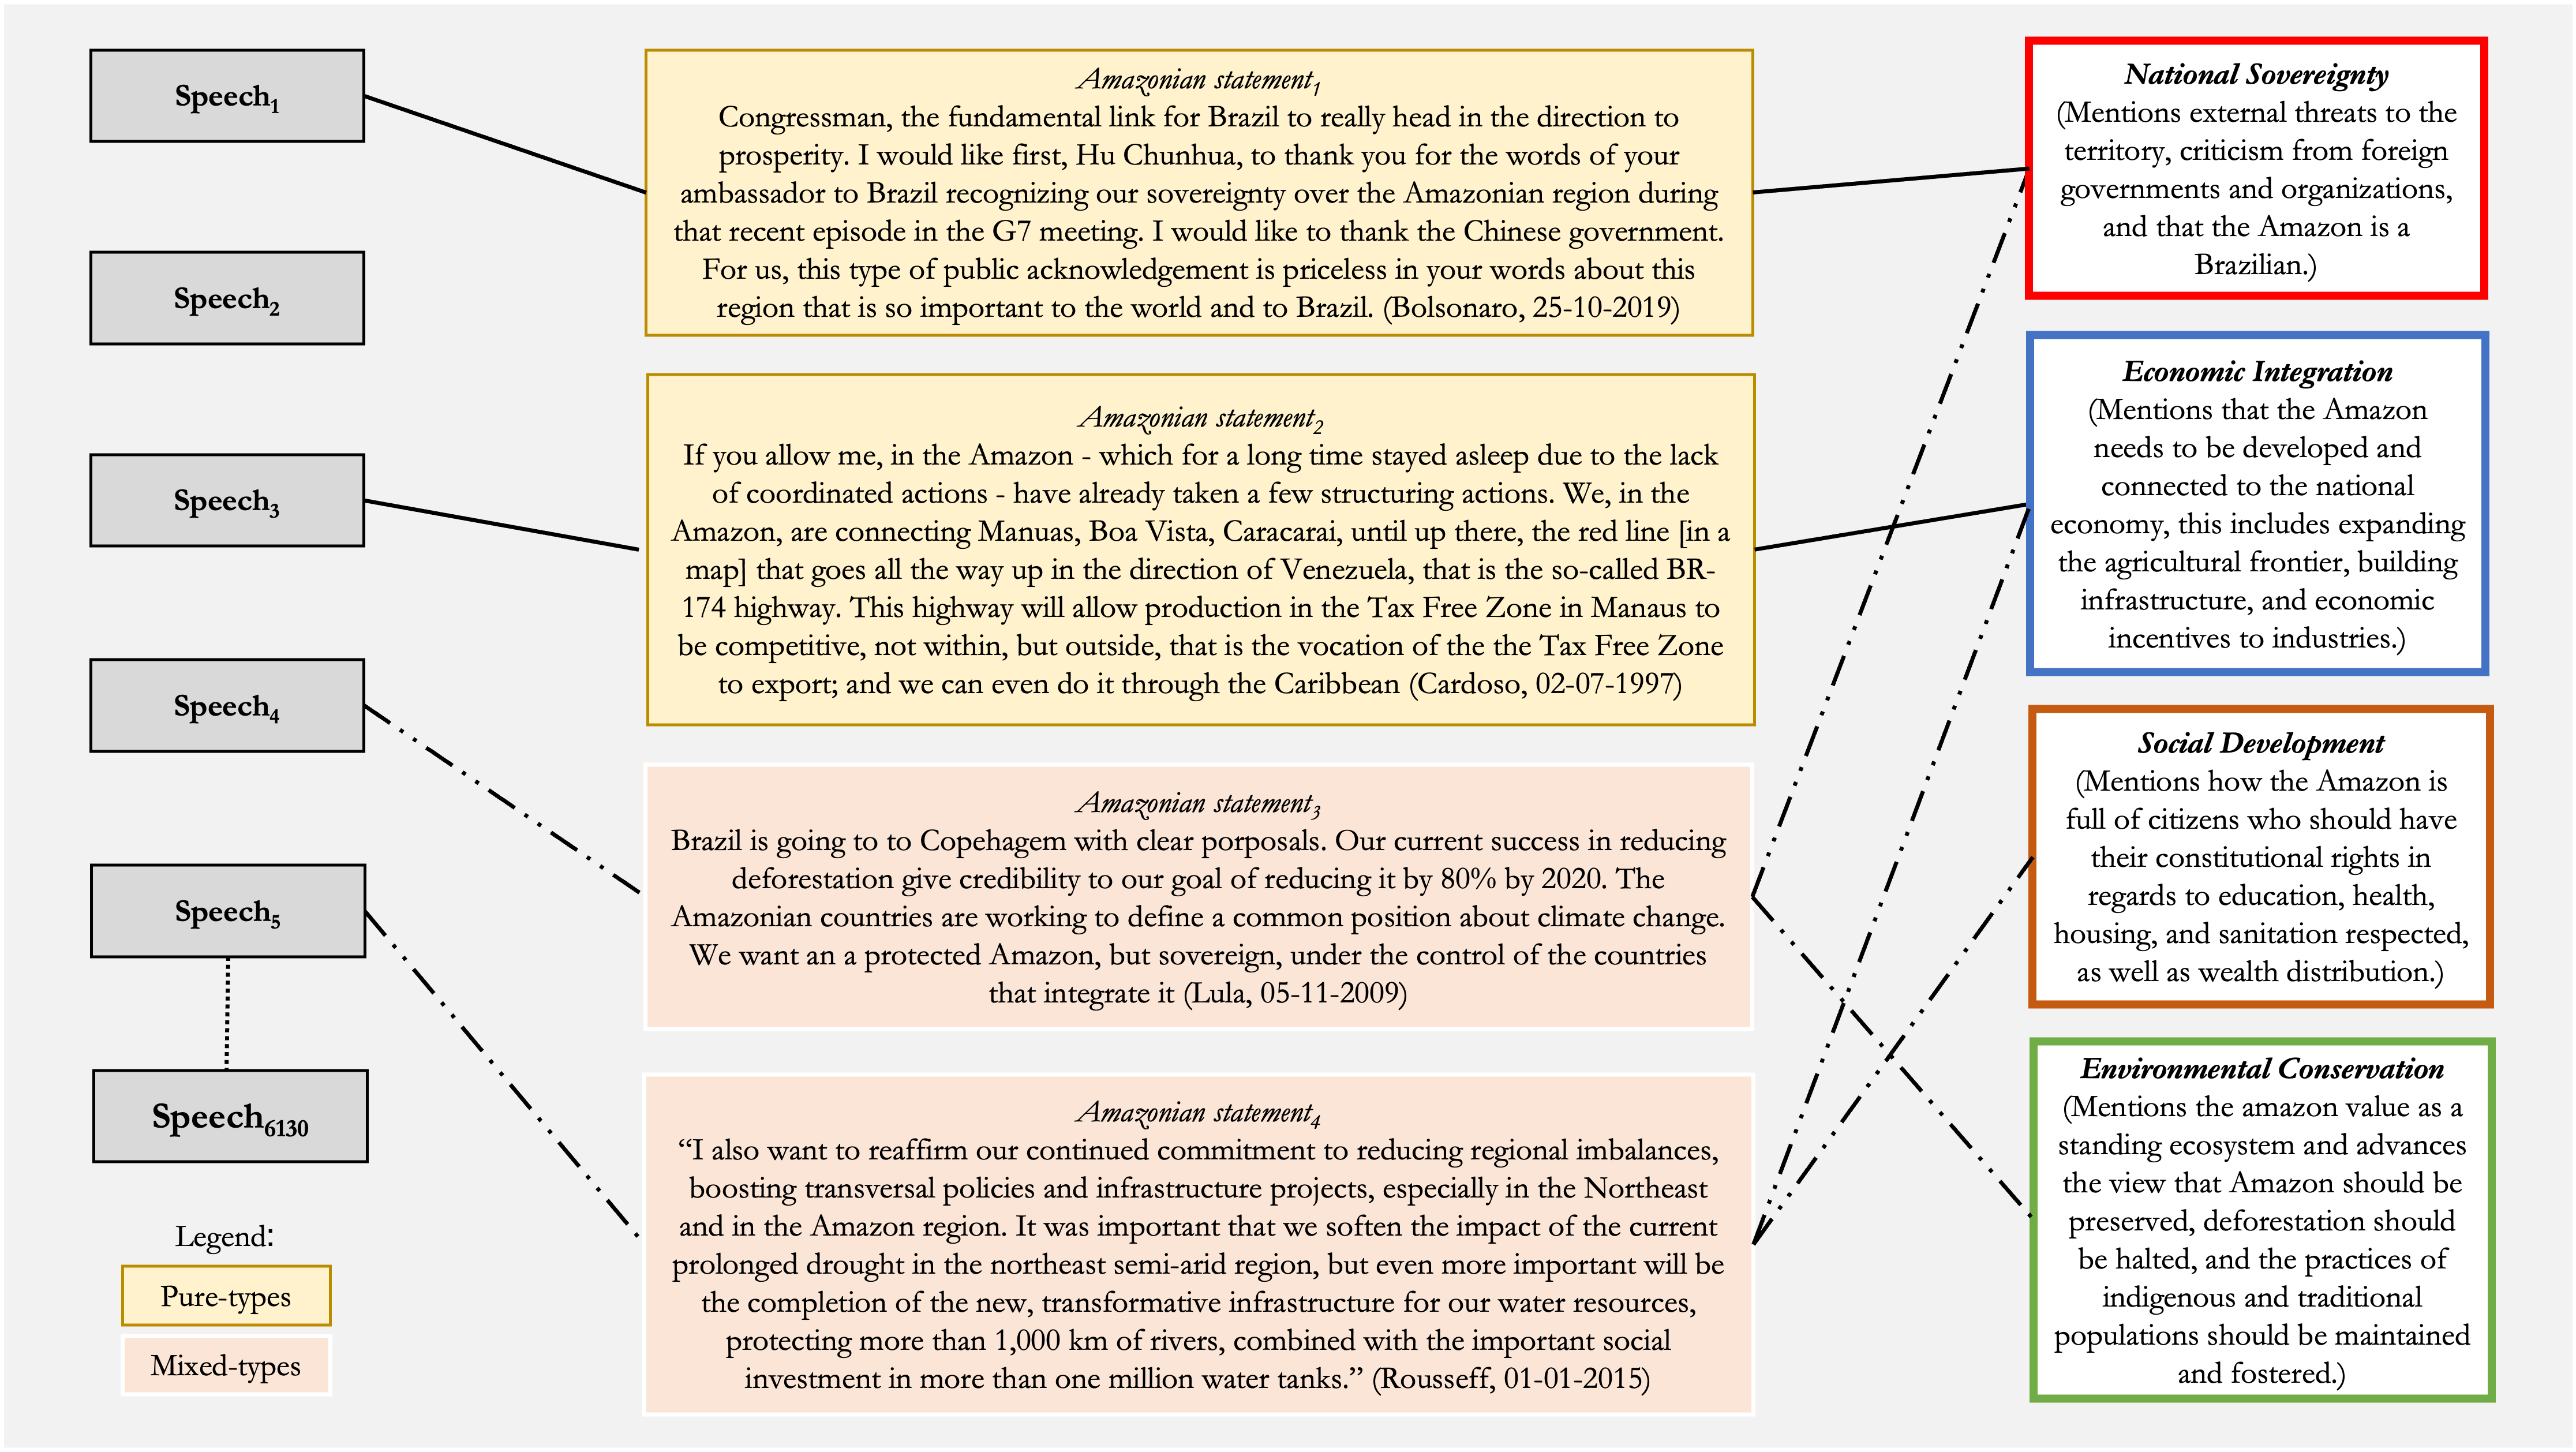
\includegraphics[width=1\linewidth]{figure1pic} \caption{Operationalization of problem-constructions}\label{fig:figure1}
\end{figure}

\end{landscape}

Second, with the codebook in hand, each one of the authors, separately,
hand-coded the same set of 1007 randomly selected Amazonian statements.
This amount refers to 50\% of all the Amazon Statements identified. We
chose to hand code half of the observations because since there are
several nuances in discourse in how presidents talk about the amazon in
time and as a problem, we conservatively code a relatively large
training set for the subsequent automated machine learning. As well,
this allows a robust validation set to verify the models. As the size of
the training set should increase with the number of categories (Grimmer,
Roberts, and Stewart 2022), we deemed four categories and 50\% of the
statements as reliable enough. Also, automating the coding of half of
the observations saved the authors over one month of work in comparison
to manual coding. Intercoder agreement for each of the four main
categories was 85\%, on average. For each non-matching coded
observation, the co-authors discussed and sorted their disagreements.

Third, the hand-coded data is then randomly divided into a training set,
containing 80\% of the hand-coded observations (806 observations), and a
validation set, containing the remaining 20\% of the hand-coded data
(201 observations). We chose to employ a support-vector machine (SVM)
algorithm to label texts, that is, a non- probabilistic linear
classifier that classifies documents by assigning points in mapped space
to maximize the gap between binary categories (Meyer et al. 2021; Noble
2006) . The SVM model is first trained using the hand coded training set
and then employed to classify observations in the hand coded validation
set. The trained SVM model was, on average 82\%, accurate in classifying
observations in the validation set before being tuned. After the SVM
model is tuned, we use the model to automatically code the remaining
1007 Amazonian statements. The final dataset for analysis, excluding
false positive matches, contains 1895 coded Amazonian statements.
Finally, we extract locations for all speeches in the data. These
locations represent the Brazilian state in which certain speech was
given or an international country.

\hypertarget{analysis-and-limitations}{%
\subsection{3.2 Analysis and
Limitations}\label{analysis-and-limitations}}

To analyze our data, we first present a series of different plots on
proportions of Amazonian statements and problem-constructions over time
and by presidents. To test whether different problem constructions
change according to location, we run a multinomial logit model in which
different problem constructions (as categories) are the dependent
variable and location is the independent variable. Multinomial logit is
an appropriate method for modeling data in which the dependent variable
of interest is categorical, unordered, and has many categories, as is
our case (Kwak and Clayton-Matthews 2002). In our model, we also control
for annual deforestation rates, annual inflation rates, and election
years in the model. We interpret the plots and model considering
multiple Amazon related events and policies over the last 30 years, as
well as their correlations with different presidents and locations,
while embedding problem-construction in contemporary happenings.

This approach also comes with limitations. Our codebook is developed
using specific Amazon-related vocabulary. For example, a statement will
be coded as economic integration if it is meaningful support to the
tax-free zone of Manaus or a Dam in the Amazon. However, the economy is
generally a topic that presidents speak about. Hence, the high incidence
of economic integration in Amazonian statements can also be related to
the higher importance of this problem-construction in Brazil in time.
Moreover, we classify statements as Amazonian based on a dictionary
composed of a single lexicon stem: ``amazon''. We chose to do so knowing
that a few speeches about the Amazon might not contain the lexicon
``Amazon'', for example, when the president says, ``the forest'' or
``deforestation''. Hence, we might be missing statements about Amazon
that do not refer to it. However, we consider this safer as we cannot be
sure that mentions of the forest or deforestation do not correspond to
other biomes such as the Cerrado or the Mata Atlantica. Nevertheless,
our dataset covers only what is considered an official remark.
Presidents, though, give interviews, appear in debates, talk at campaign
rallies, and more recently started to appear on social media. Problem-
construction within presidential discourse, thus, also happens in
different sites for which we do not account for in this paper.

\hypertarget{the-amazon-in-presidential-speeches}{%
\section{4 The Amazon in Presidential
Speeches}\label{the-amazon-in-presidential-speeches}}

\hypertarget{the-rises-and-falls-of-the-amazon-as-a-topic-in-presidential-speeches}{%
\subsection{4.1 The rises and falls of the Amazon as a topic in
presidential
speeches}\label{the-rises-and-falls-of-the-amazon-as-a-topic-in-presidential-speeches}}

The frequency in which the Amazon appears across all official
presidential speeches varies in time. Figure 2, below, shows the
proportion of speeches that mentions the Amazon in relation to all
speeches per year. We observe five local maxima: 1989, 1992, 2009, 2015,
and 2019. These points, usually, coincide with events that help us
explain the rises and falls of the Amazon in presidential discourse in
time. For instance, in 1985 the Amazon appeared in about 4\% of all the
presidential speeches but by 1988 this had increased to around 14\%.
This is the period when the Brazilian Constitution was written.
Indigenous and traditional populations were instrumental in advocating
for constitutional environmental rights and the protection of their
territories (Hecht and Cockburn 1990). These were eventually enshrined
in article 225, which gives all Brazilians a right to a balanced
environment, and in article 231, which grants indigenous and traditional
populations a right over their territory. However, in 1989, the Amazon
appeared in 32\% of all speeches. This spike is likely explained by the
brutal murder of Chico Mendes and the very end of 1988. An incident that
caught unprecedented international attention and Sarney responded to
this with a set of policies to address deforestation (Capobianco 2021).

\begin{figure}
\centering
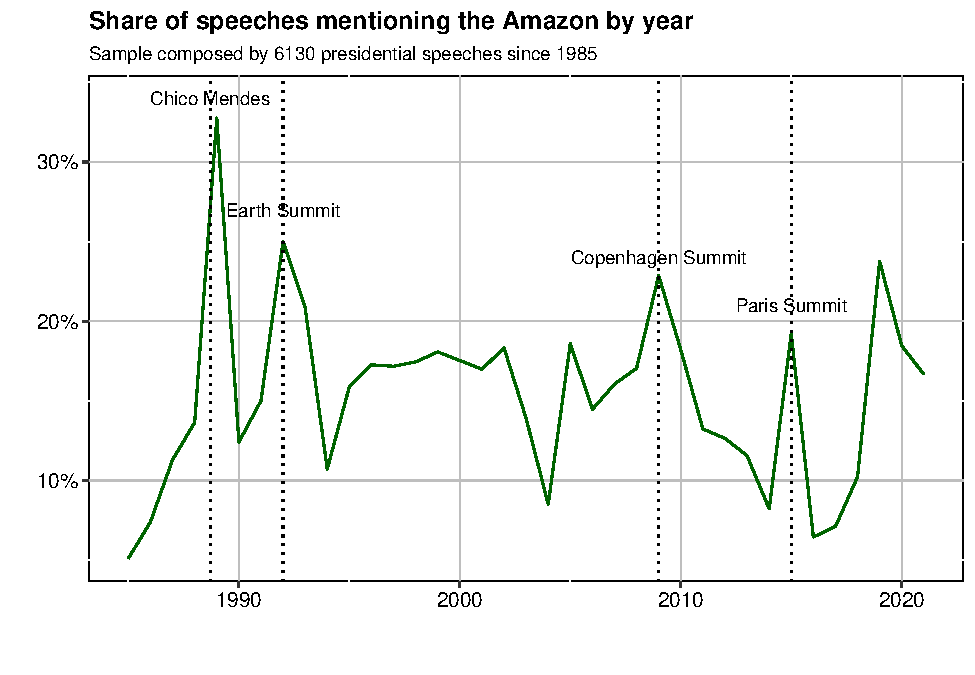
\includegraphics{Full_draft_20220608_files/figure-latex/Figure 2-1.pdf}
\caption{Amazonian speeches by year}
\end{figure}

In 1990 the Amazon appeared in 12\% of all speeches and, by 1992, this
increased to 25\% of all speeches. The 1992 Earth Summit, held in Brazil
brought international attention to environmental topics in the Amazon.
One of the big announcements, for example, was the consolidation of the
first transnational partnership for the Amazon, the G7 Pilot Programme,
which brought a high number of financial resources to the region for
public policy implementation (Capobianco 2021). Throughout the 1990s and
2000s, during the Cardoso and Lula administrations, the Amazon appeared,
on average, on 15\% of all speeches. Exceptionally, in 2009 we see
another spike in the Amazon appearing in official speeches. This spike
coincides with the 2009 Copenhagen Summit as well as the steepest
decrease in deforestation rates since data is available. Lula led the
delegation to Copenhagen with a self-image of ``we do not promise, we
deliver'' when the stakes about climate change were high (Franchini and
Viola 2019).

From 2010 to 2018, with the exception of 2015, we see a general decrease
in mentions of the Amazon in all official presidential speeches. From
2010 to 2014, mentions of the Amazon went down from 18\% to 8\% in
official speeches. Disagreements related to the priority of
environmental preservation over economic development, most notably in
the case of Itaipu Dam, led the environmental minister Marina Silva to
resign and run for the presidency on her agenda in 2010. In 2011, the
New Forest Code, which regularized land ownership of many illegally
deforested areas, was also approved. These are also the years when
Brazil entered a long period of political and economic instability,
which eventually led to the impeachment of Dilma Roussef. Though, in
2015, the Amazon appeared in 19\% of speeches. This spike coincides with
the Paris summit which became a key turn in climate politics after the
failures of Copenhagen. Brazil went to the Paris Summit with
deforestation numbers slightly higher than Copenhagen and a perception
that there was a turn towards less conservation. By 2016 mentions of the
Amazon in official speeches went down to 6\%, the lowest share since
1985.

We subsequently observe a steady increase from 6\% in 2016 to almost
24\% in the first year of Bolsonaro's presidency, 2019. At the time,
international and national media brought unprecedented attention to
Brazilian environmental issues as the record burning of the Amazon, and
of the red sky afternoon in São Paulo circulated on social media and
international media outlets. This brought issues related to
environmental conservation as high priorities in Bolsonaro's governing
agenda with efforts to dismantle key pillars of Brazilian environmental
governance. At the same time, President Bolsonaro retrieves Brazil's
hosting status for COP25. In short, relevant international events drive
interest and alter how pressing the ``Amazon problem'' is perceived to
be in society, therefore, cause a momentary shift of interest from top
policymakers.

\hypertarget{how-has-the-amazon-been-constructed-as-a-problem}{%
\subsection{4.2 How has the Amazon been constructed as a
problem?}\label{how-has-the-amazon-been-constructed-as-a-problem}}

\hypertarget{pure-type-problem-constructions}{%
\subsubsection{Pure-type problem
constructions}\label{pure-type-problem-constructions}}

We conceptualize four pure problem constructions: sovereignty, economic
integration, social development, and conservation. At the level of the
speech, though, presidents might mix multiple problem construction in an
Amazonian statement. Figure 3, below, illustrates the share of each pure
type in time. Pure problem constructions dominate, with an average of
56\% of all amazonian statements across time. As above, we observe a
strong variation over time for most of these constructions.

\begin{figure}
\centering
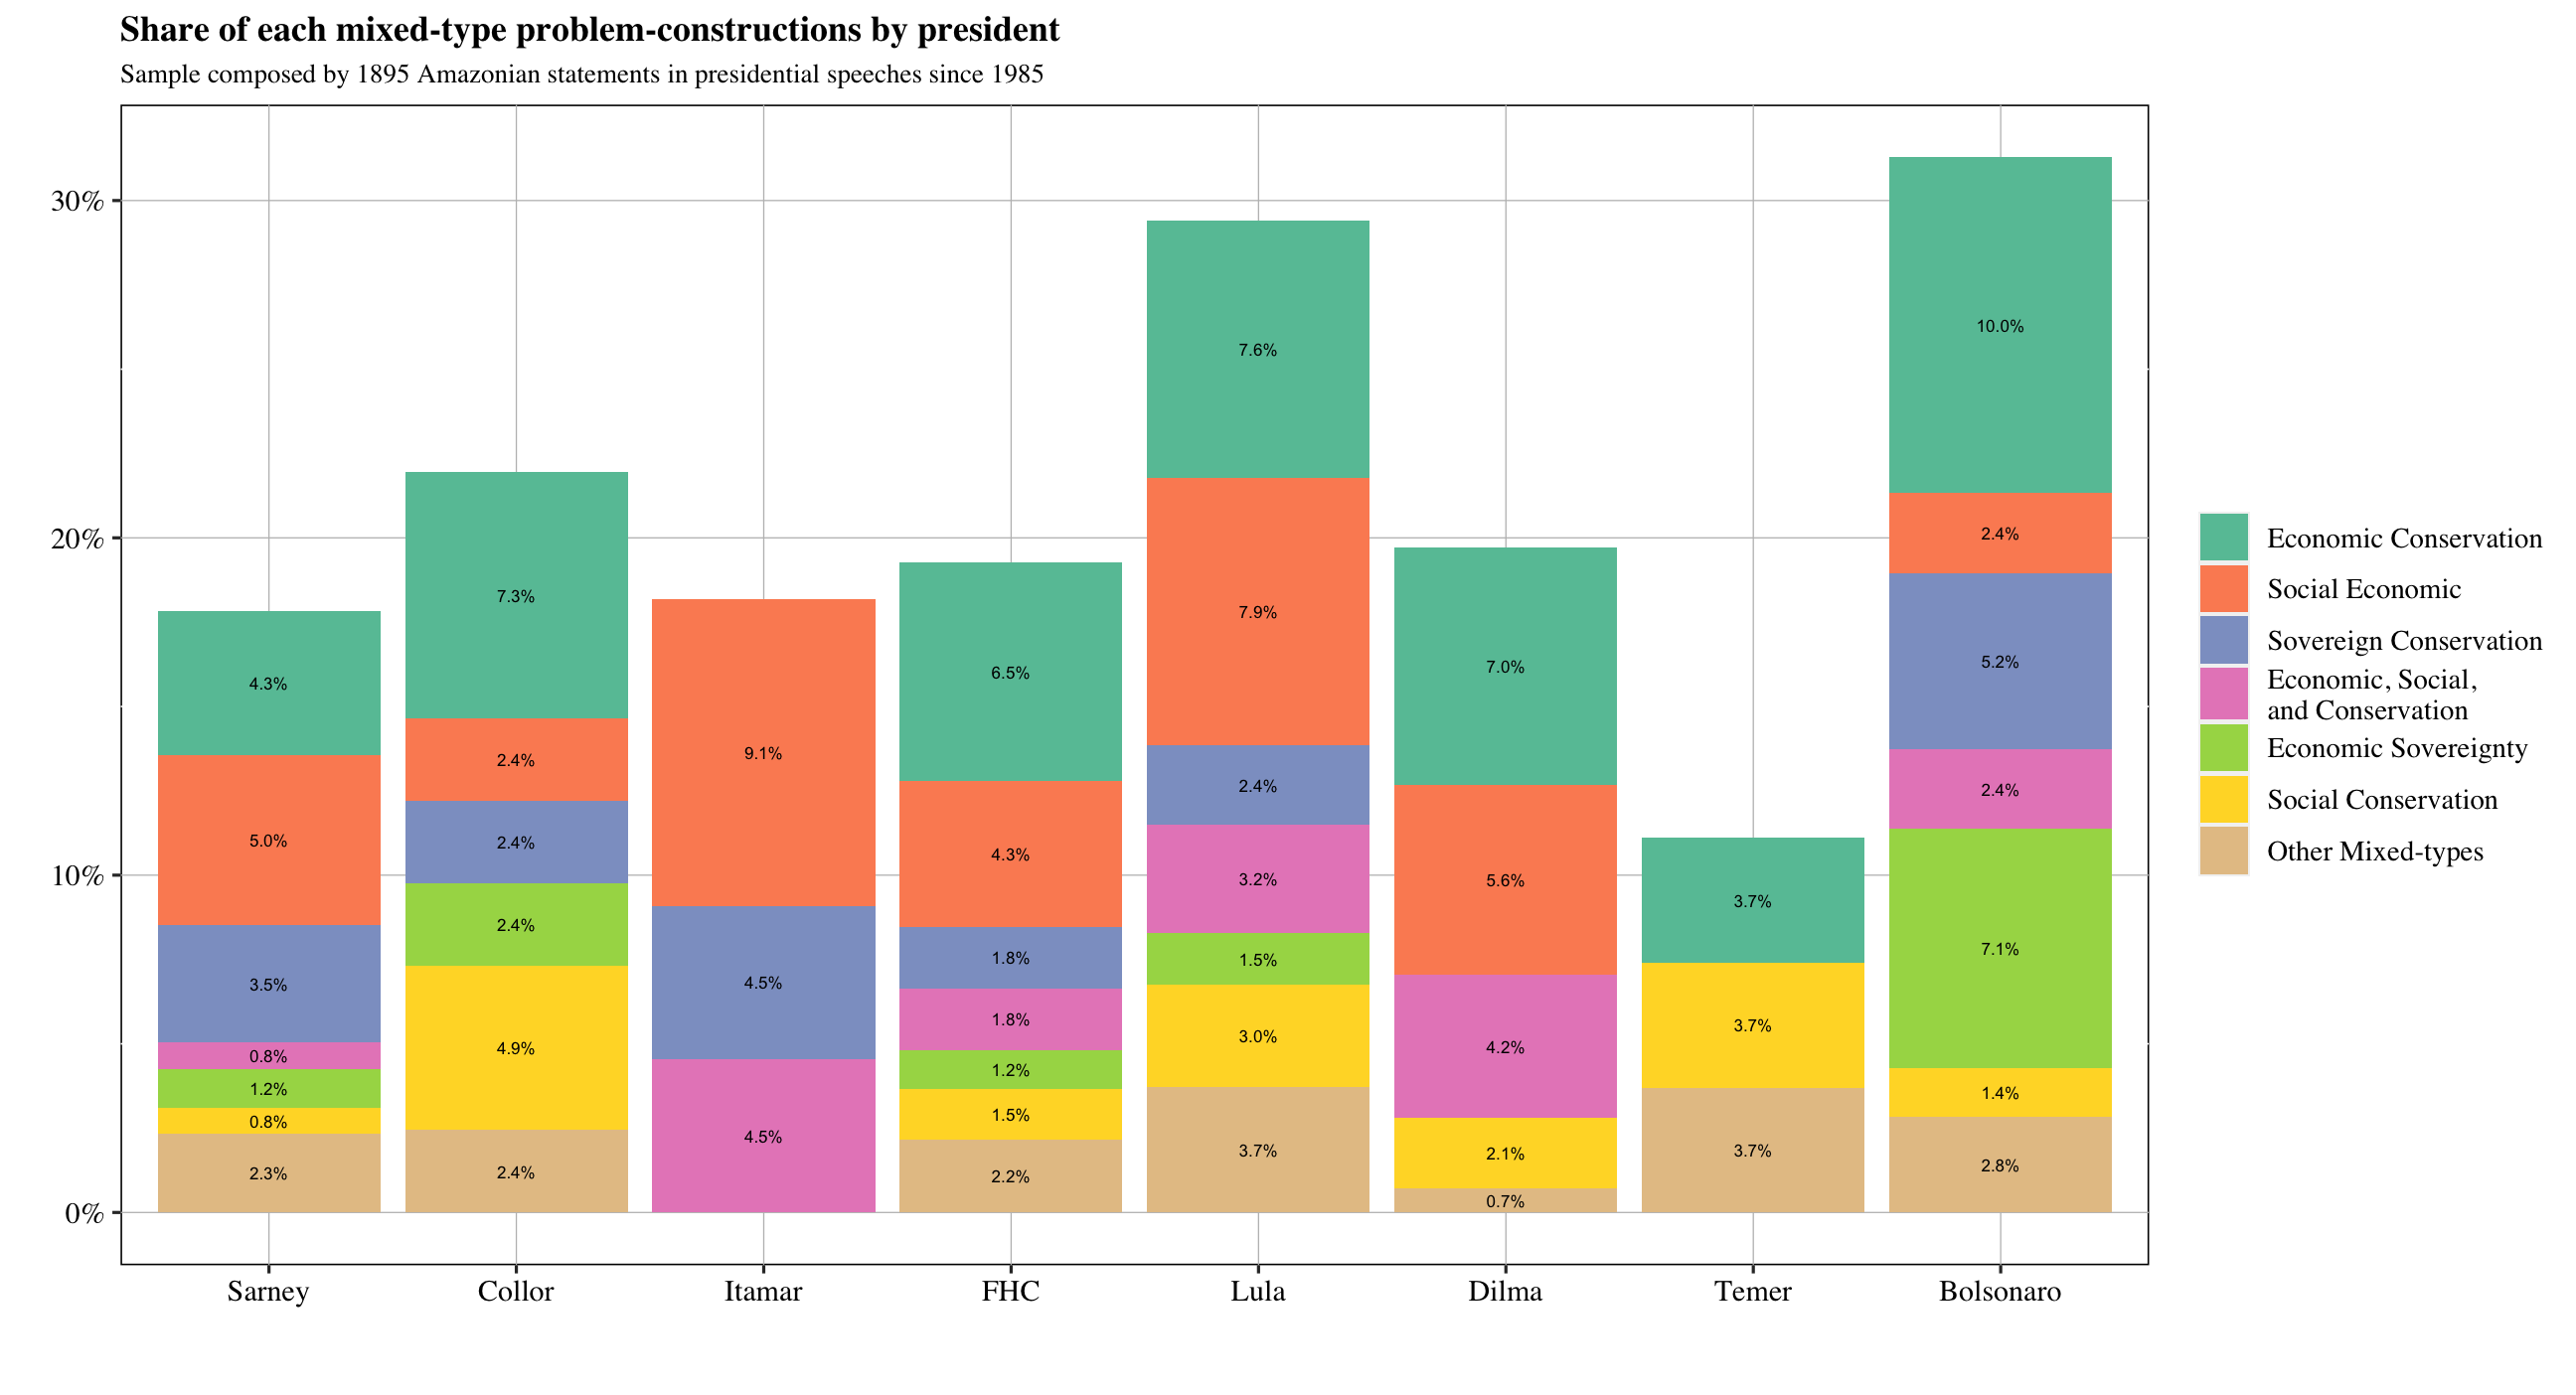
\includegraphics{Full_draft_20220608_files/figure-latex/Figure 3-1.pdf}
\caption{Pure types in time}
\end{figure}

Amazonian constructions are not monolithic in time nor within
governments. The same governments construct the Amazon as different
issues in discourse. Pure economic integration constructions dominated
constructions from 1985 to the late 2000s. This is especially pertinent
during the Cardoso administration as the Amazon was constructed,
overwhelmingly, as an issue of economic integration. However, during
Lula's terms in office, constructions of the Amazon purely as an
economic issue decreased in discourse while constructions of the Amazon
as issues of pure conservation as well as of pure social development
increased. These constructions surpassed economic integration around
2010. These trends in discourse continued during the Rousseff
administration. Capobianco (2021), for example, argues that the
unprecedented decrease in deforestation we observed from 2004 to 2012
was a product of an increase in the perception of stronger federal
policies and presence in the Amazon region, which in turn engendered a
perception of higher risk of being caught and fined for deforestation. A
higher incidence of the Amazon, as a topic in overall presidential
speeches, generates a perception that more attention is being paid to
the Amazon from the top while the shift from constructing the Amazon as
an issue of economic integration to an issue of environmental
conservation generates a perception that illegal deforestation will be
increasingly monitored.

From the mid-2010s onwards, we start to see a reverse of this trend:
economic integration problem construction increases while conservation
and social development constructions decrease instead. Interestingly,
sovereignty starts to increase steadily from 2010 onwards and by 2019
sovereignty constructions surpass social development. Figure 3 also
highlights that, while the reversal precedes the mandate of President
Bolsonaro, it was with him that sovereignty constructions reached
unprecedented levels since the establishment of Brazilian democracy.

\hypertarget{mixed-type-problem-constructions}{%
\subsubsection{Mixed-type problem
constructions}\label{mixed-type-problem-constructions}}

Although presidents prefer pure problem-constructions, they also
construct the Amazon as multifaceted issues. Mixed-type problem
constructions in discourse offer more complex understandings of the
Amazon as an issue. Constructing the Amazon as multiple issues averages
at 18\% of all constructions in time. While there is some variation in
time, some mixed-types rarely appear, thus, we focus our discussion on
those mixed-types with higher incidence. Figure 4, below, displays the
average mixed-types by president.

\begin{figure}
\centering
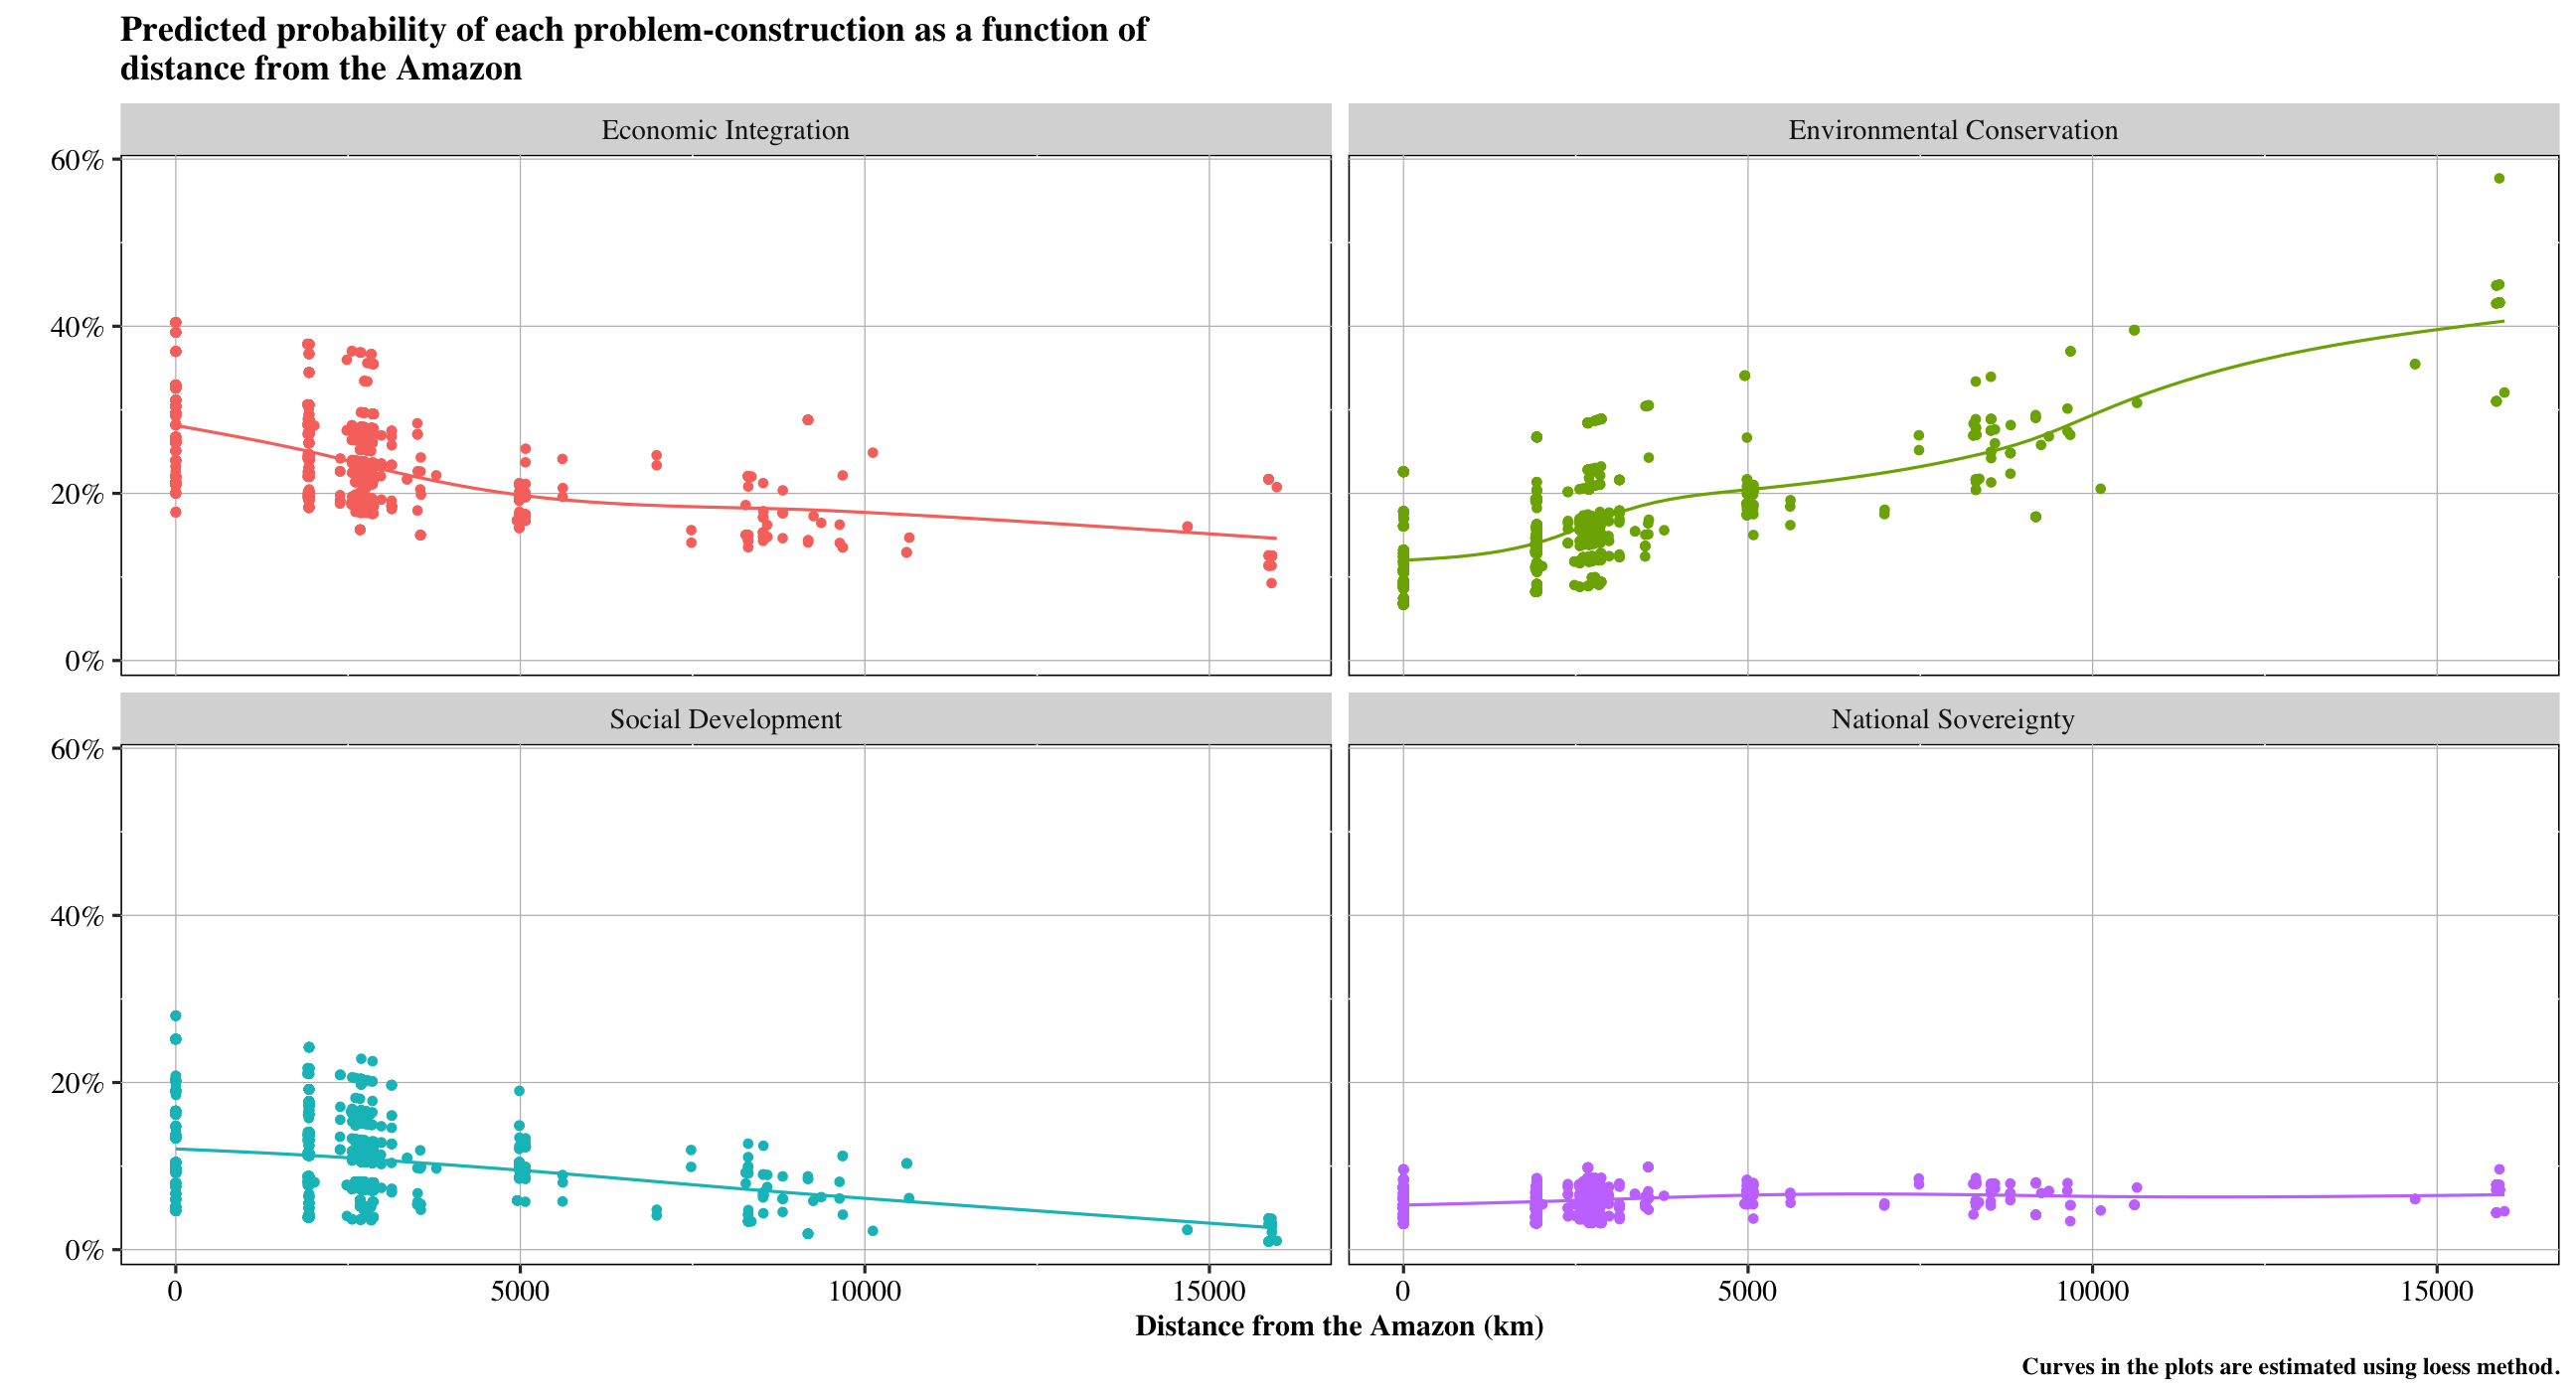
\includegraphics{Full_draft_20220608_files/figure-latex/Figure 4-1.pdf}
\caption{Mixed-types by president}
\end{figure}

The most frequent mixed-type problem construction of the Amazon in time
is economic corsevation. The mixed-type is composed of Amazonian
statements that construct the Amazon as problems of both economic
integration and environmental conservation. Economic conservation
averages at 6.8\% in relation to all Amazonian statements. The mixed
type generally increased in time, with Bolsonaro employing the
mixed-type higher than all other presidents. The second most common
mixed-type in time mixes social development and economic integration and
appears, on average, in 5.4\% of all statements. Notoriously, Lula
employs such a mix-type more frequently than all other presidents. In
fact, both Lula and Bolsonaro construct the Amazon as multifaceted
issues in discourse more frequently than other presidents. While Lula,
on the one hand, often mixes economic integration with environmental
conservation and social development when constructing the Amazon as an
issue, Bolsonaro, on the other hand, often mixes national sovereignty
with other problem constructions. Indeed, we see that Bolsonaro
constructs the Amazon as an issue of national sovereignty and economic
integration more than any other president, which was also characteristic
of the military dictatorship discourses and policies for the region
(Hecht and Cockburn 1990).

\hypertarget{the-amazonian-multi-level-game-boasting-policy-outside-and-talking-to-people-inside}{%
\subsection{4.3 The Amazonian multi-level game, boasting policy outside
and talking to people
inside}\label{the-amazonian-multi-level-game-boasting-policy-outside-and-talking-to-people-inside}}

Problem constructions depend on where presidents speak. To facilitate
analysis and make sense of locations, we divide locations into Amazonian
states (i.e.~all the Brazilian states in which the Amazon biome is
present), non Amazonian states (other Brazilian states), Brasilia (the
capital of Brazil where the federal government is located), Amazonian
countries (neighboring countries where the biome is present), and
international countries (countries outside of Brazil). To analyze the
relationship between location and problem construction, we run a
multinomial regression. Our dependent variable is problem-constructions
(categorical), while our main independent variable is location
(categorical). The reference category for the multinomial model is,
thus, environmental conservation in international states. We control for
deforestation rates (numerical), inflation (numerical), and election
year. Since the model accounts for both mixed and pure-type Amazonian
constructions, and this makes for a large table, we focus the analysis
on pure-types to facilitate visualization (see full regression table in
appendix).

Figure 5, below, shows the percentage of problem-constructions by
location derived from the regression model. The plot illustrates the
percentage likelihood of constructing the Amazon as a certain issue
according to location in relation to the reference category,
environmental conservation internationally. From the figure we see, for
example, that presidents are 29\% more likely to construct the Amazon as
an issue of economic integration within other Amazonian countries in
comparison to other international settings. Although without the same
strength, the finding also holds at the state level within Brazil as
presidents are 11\% more likely to construct the Amazon as an issue of
economic integration within Amazonian states and 15\% more likely in non
Amazonian states. Interestingly, presidents are less likely to construct
the Amazon as an issue of economic integration in Brasilia than
internationally. That is, when speaking internationally or in Brasilia,
presidents often construct the Amazon as an issue of environmental
conservation.

\begin{figure}
\centering
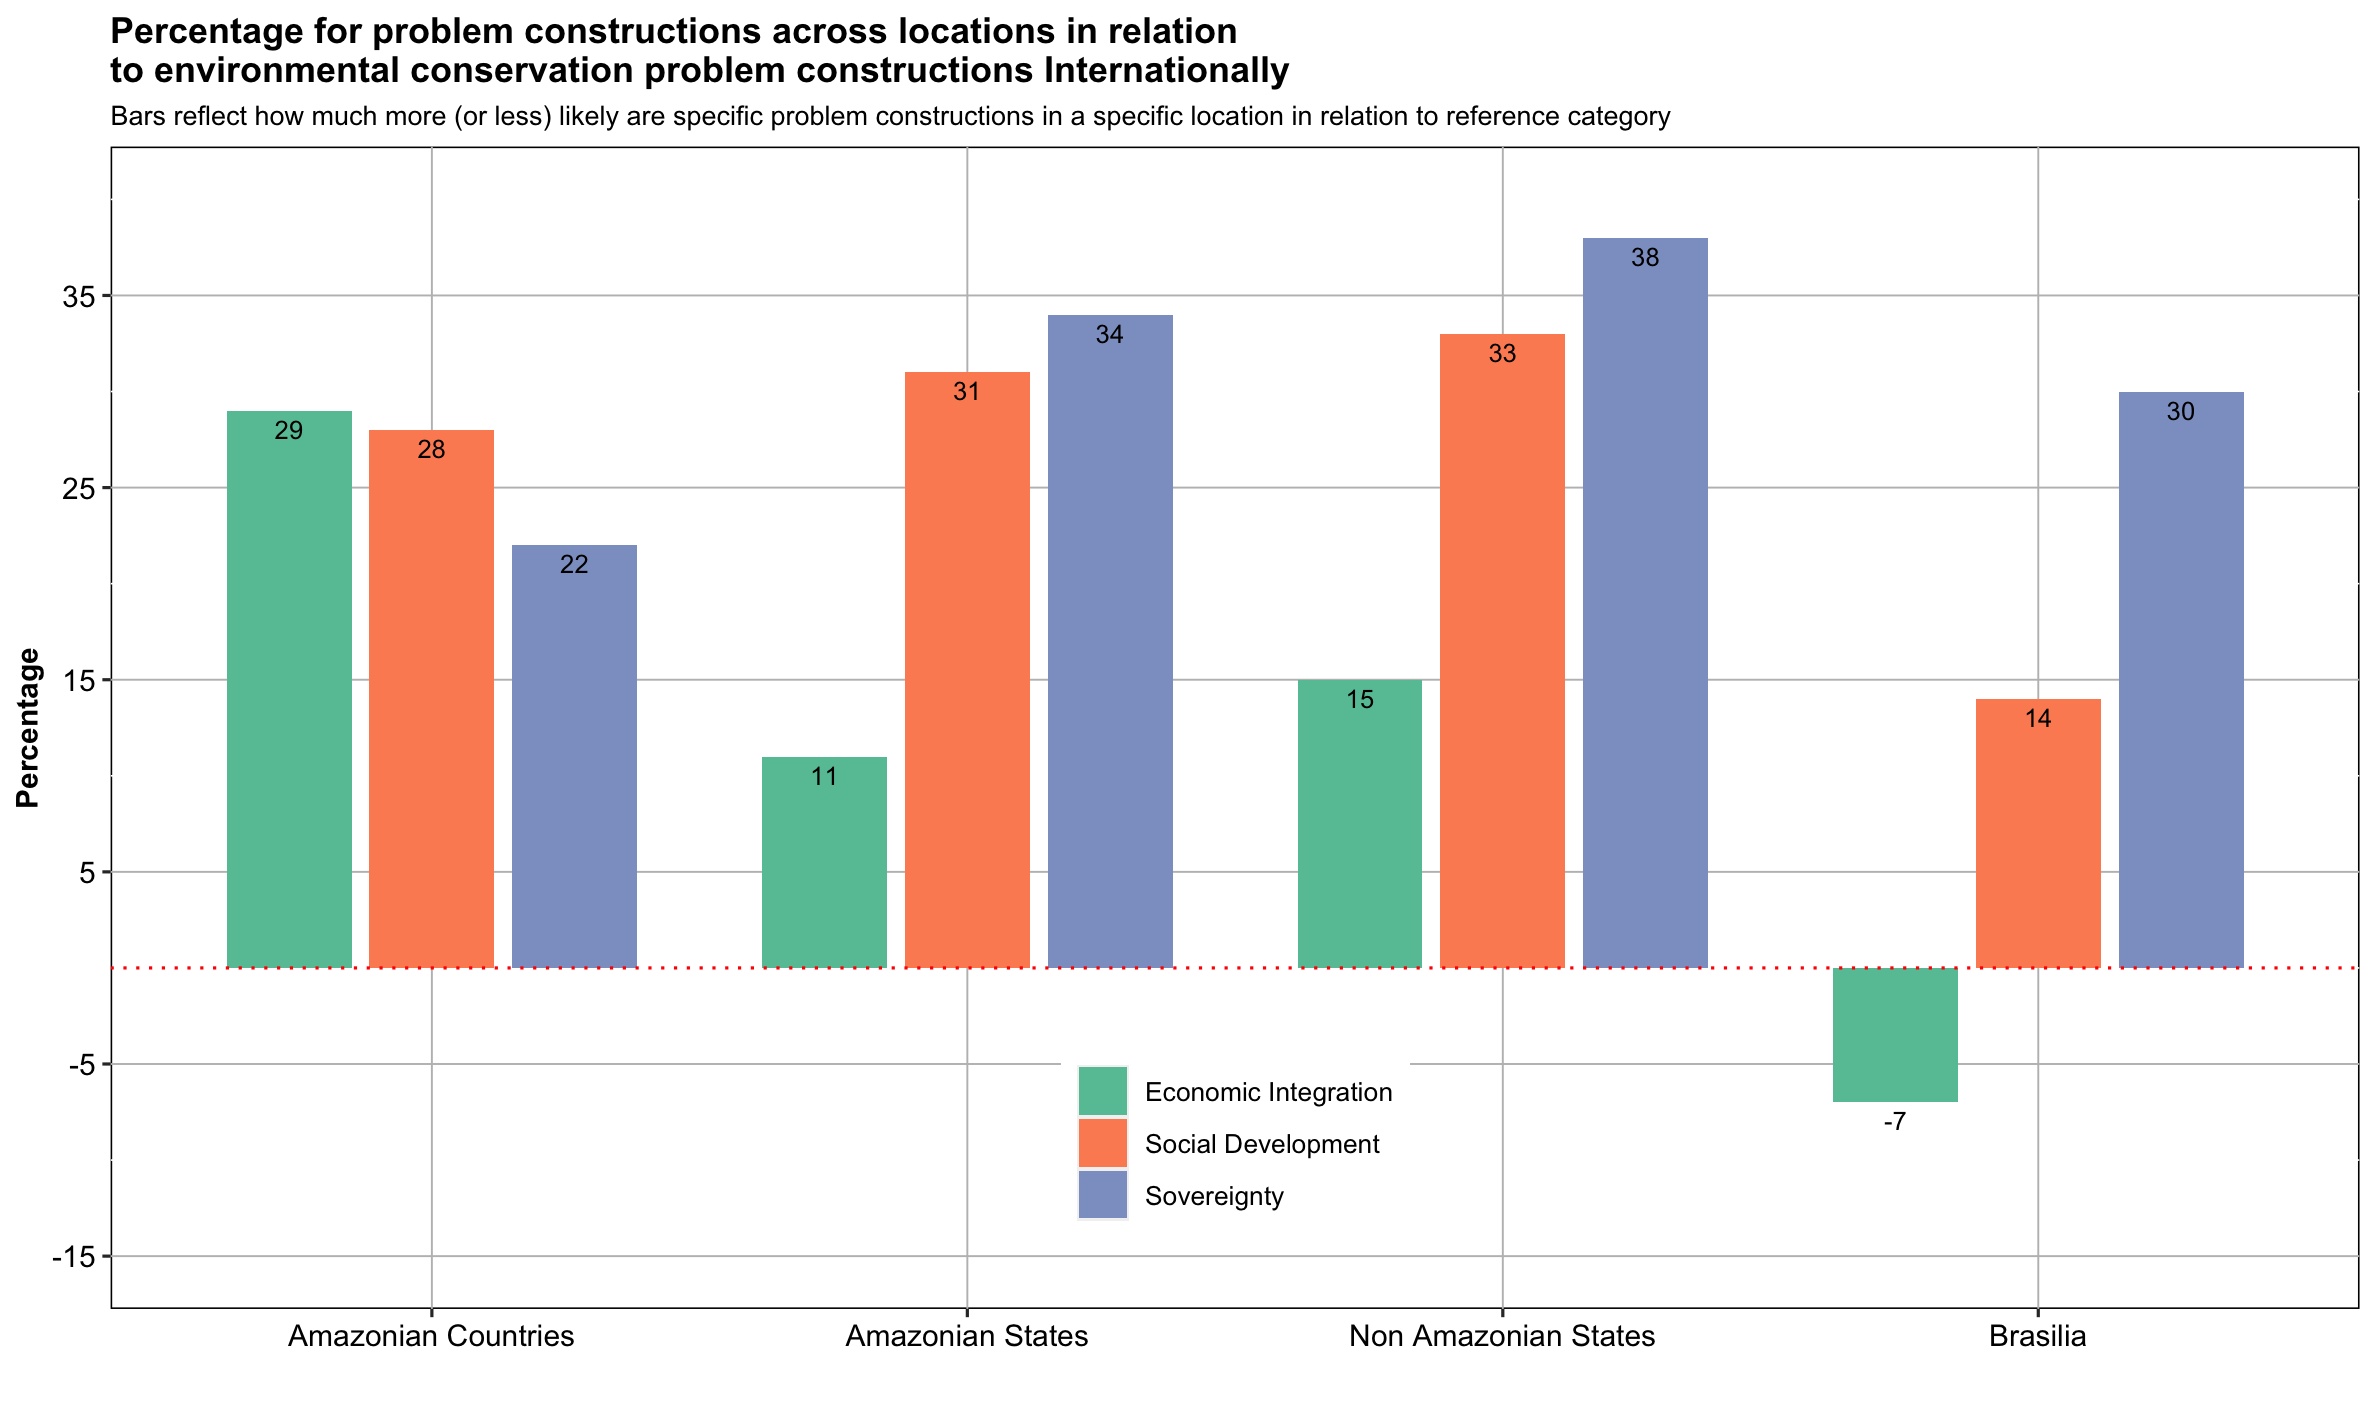
\includegraphics{Full_draft_20220608_files/figure-latex/Figure 5-1.pdf}
\caption{Percent of problem constructions across locations}
\end{figure}

Along these lines, constructing the Amazon as an issue of social
development takes place, overwhelmingly, within Brazil or other
Amazonian countries. Presidents are at least 14\% more likely to
construct the Amazon as an issue of social development in these
locations than internationally. The same is true for sovereignty,
whereas constructing the Amazon as an issue of sovereignty takes place
within Brazil or in neighboring Amazonian countries. Notice, as well,
how Amazonian constructions within Amazonia states and non Amazonian
states are strikingly similar. This indicates that presidents are
consistent when constructing the Amazon locally across the federation,
when outside of Brasilia.

How the amazon is constructed as a problem varies across levels. The
Amazon, as a region and a forest, has historically been the topic of
international, national, supranational, and local debates, negotiation
and policies. This implies not only that audiences' priorities in each
setting change, but that which policies are appropriate to solve the
``Amazon issue'' could differ as well. The multi-level game entails that
conservation might be a desirable construction when speaking
internationally about the Amazon, or in Brasilia, but not for local
electorates. Local electorates who, ultimately, elect presidents. This
multi-level game leads to different policies being negotiated, often
simultaneously, so that the overlap at the interplay between the levels
is maximized. Take, for once, how the Brazilian government successfully
funded domestic public policy with international support since the 1990s
(e.g.~1992 Programa Piloto para Proteção das Florestas Tropicais), by
creating a federal fund for the protected areas (e.g.~2001 Amazon Region
Protected Areas program), and by assuring international funds with the
establishment of the Amazon Fund in 2008 which provided over USD 1
billion for environmental conservation in the Amazon (Silva-Muller and
Faul 2022). Still, this does not mean, though, that the national agenda
of economic integration or social development was not pursued. During
the same time rural credit offered to local agricultural producers in
Amazonian states, went up from 500 million reais a year in 1999 to over
4 billion a year by 2012 (Capobianco 2021). Nowadays, it has reached
unprecedented levels.

\hypertarget{discussion-and-conclusion}{%
\section{5 Discussion and Conclusion}\label{discussion-and-conclusion}}

The Amazon frontier as an analytic category can help us shed light on
the differences we identify between the discourse within Brazilian
states and Amazonian countries compared to Brasilia or internationally.
Whereas presidential discourses at the top matter to define and justify
public policy (Zarefsky 2004), presidents shape their discourses
according to who their audience might be and what ``they want to hear''.
If presidents promote an agenda of economic and social development
within Brazil that diverges from the one the president promotes outside
of Brazil, the question for democracy becomes to what extent the
implemented agenda responds to domestic versus international demands.
Or, as Putnam (1988) puts it, what's the actual overlap between the
international and domestic overlap. The domestic policies and
transnational support that led to the decrease in deforestation from
2004 to 2012 happened concurrently with a period of strong economic
growth and social development in Brazil and worldwide. With the
strengthening of environmentalism and indigenous participation in
politics in the late 1980s and 1990s, we can interpret the fall of
economic integration problem-construction and the rise of social and
conservation constructions as a new balance between granting local
livelihoods their rights and economic exploitation.

While unprecedented, this new balance was not long-standing. Democratic
decay is slow, and the embryo of Bolsonaro's Amazonian discourse was
breeding half a decade before he took office. We observe the decrease in
conservation-related statements in the mid-2010s, and a hard increase of
sovereignty constructions in the early 2010s. As we conceptualize and
operationalize sovereignty as boundary-making vis- à-vis internal and
external perceived threats to the Amazon, we interpret this increase as
not only attacks to international interference in the Amazon but also on
indigenous and traditional populations. On the policy side, the Itaipu
Dam in the late 2000s and the 2011 Forest code is seen as a turning
point: political opposition to conservation got particularly organized
and managed to lobby the executive and conquer this policy wins, which
were largely opposed by environmentalists. The political forces in
Brazilian democracy that drive these changes in problem-construction
were long in the making, as the earlier and softer shifts in discourse
suggest. Bolsonaro's problem-construction is the strongest form of this
shift.

In sum, this paper investigates how the Amazon has been constructed as a
problem in Brazilian presidential speeches since 1985. Our findings show
that these constructions are not monolithic within governments, in time,
or across different locations. Conceptually, this contributes to
understanding the social construction of the Amazon in discourses and
how these might relate to policies and environmental outcomes.
Empirically, we provide the first comprehensive overview of the Amazon
in presidential discourse. Given the importance of discursive
problem-construction within democracies to legitimize ways of thinking
and acting towards the environment, further research on the relationship
between the social construction of the Amazon, one of the worlds most
important standing ecosystems, and its effects on environmental outcomes
is pressing.

\hypertarget{appendix}{%
\section{Appendix}\label{appendix}}

\begin{landscape}

\begin{table}

\caption{\label{tab:codebook}Amazonian Problem-Construction Codebook}
\centering
\resizebox{\linewidth}{!}{
\fontsize{9}{11}\selectfont
\begin{tabu} to \linewidth {>{\raggedright\arraybackslash}p{3cm}>{\raggedright\arraybackslash}p{9cm}>{\raggedright\arraybackslash}p{9cm}}
\toprule
Problem Construction & Description & Example\\
\midrule
\textbf{\cellcolor{gray!6}{National Sovereignty}} & \cellcolor{gray!6}{This code constructs the Amazon region and/or forest as an issue of national sovereignty. We understand claims of sovereignty as a particular problem-construction that touches on imaginaries of external threats to territory. Relatedly, we also understand sovereignty as raising concerns about wrong perspectives and criticism from foreign and non-state actors about governments<U+2019> actions related to the Brazilian Amazon. In all, it advances the view that the Amazon is Brazilian, foreign, and non-state presence in the region needs to be monitored closely.} & \cellcolor{gray!6}{Congressman, the fundamental link for Brazil to really head in the direction to prosperity. I would like first, Hu Chunhua,  to thank you for the words of your ambassador to Brazil recognizing our sovereignty over the Amazonian region during that recent episode in the G7 meeting. I would like to thank the Chinese government. For us, this type of public acknowledgement is priceless in your words about this region that is so important to the world and to Brazil. (Bolsonaro 25/10/2019)}\\
\textbf{Economic Integration} & This code constructs the Amazon region and/or forest as an issue of economic integration. It advances the view that the Amazon needs to be developed and connected to the national economy. This includes expanding the agricultural frontier through incentives, creating a diverse set of infrastructure (roads, dams, internet, radio, energy), fostering differing industries (tourism, mining, cattle, agriculture and so on) through tax-free zones, as well as facilitating the exploitation of natural resources for developmental purposes. & If you allow me, in the Amazon - which for a long time stayed asleep due to the lack of coordinated actions - have already taken a few structuring actions. We, in the Amazon, are connecting Manuas, Boa Vista, Caracarai, until up there, the red line [in a map] that goes all the way up in the direction of Venezuela, that is the so-called  BR-174 highway. This highway will allow production in the Tax Free Zone in Manaus to be competitive, not within, but outside, that is the vocation of the the Tax Free Zone to export; and we can even do it through the Caribbean (Cardoso 02/07/1997)\\
\textbf{\cellcolor{gray!6}{Social Development}} & \cellcolor{gray!6}{This code constructs the Amazon region and/or forest as an issue of social development. It advances the view that Amazon is full of citizens who should have their rights guaranteed. This refers to the construction of schools and universities (right to education), of hospitals (right to health), and of housing (right to house). This also includes guarantees of a dignified life with decent employment, access to water and sanitation, as well as access to electricity, internet, radio, and light. Finally, this includes referrals to culture and the right to vote.} & \cellcolor{gray!6}{The state does not work for profits, the state needs to guarantee dignity, we find that a citizen who lives in the riverside of the Amazon river, 600 kilometers from Manaus, has the right to have the electricity in their house, to owe a fridge, to owe a television where to watch the soap operas. We have invested over 14 billion reais in this program, in three and a half years. Do you know how many electrical lines we have already built? One million kilometers of lines. (Lula 20/11/2009)}\\
\textbf{Environmental Conservation} & This code constructs the Amazon region and/or forest as an issue of conservation. This problem-construction focuses on the value of a standing forest and of the preserved ecosystem in the region. The conservationist narrative advances the view that Amazon should be preserved, deforestation should be halted, and the practices of indigenous and traditional populations should be maintained and fostered. It advances the view that the emission of greenhouse gasses should be halted, that renewable energy should be supported, and that protected areas should be created. & I have put in place emergency measures, I have suspended the exports of wood logs, I have suspended the fiscal incentives and credits to projects that could damage the environment in the amazon and I have made a license mandatory to gold mining that prohibits utilizing mercury in the process. This began the restructuring of the governmental system of control and preservation of the environment, I have created the Brazilian Institute for the Environment and Natural Resources [IBAMA], which will be headed by Dr. Mesquita (Sarney 20/07/1989)\\
\bottomrule
\end{tabu}}
\end{table}

\end{landscape}

\begin{landscape}

\begin{table}

\caption{\label{tab:full regression results}Multinomial Regression Full}
\centering
\resizebox{\linewidth}{!}{
\fontsize{9}{11}\selectfont
\begin{tabu} to \linewidth {>{\raggedright\arraybackslash}m{3 cm}>{\centering\arraybackslash}m{2 cm}>{\centering\arraybackslash}m{2 cm}>{\centering\arraybackslash}m{2 cm}>{\centering\arraybackslash}m{2 cm}>{\centering\arraybackslash}m{2 cm}>{\centering\arraybackslash}m{2 cm}>{\centering\arraybackslash}m{2 cm}>{\centering\arraybackslash}m{2 cm}>{\centering\arraybackslash}m{2 cm}>{\centering\arraybackslash}m{2 cm}}
\toprule
\textbf{\cellcolor{gray!6}{Dependent Variable}} & \cellcolor{gray!6}{EI} & \cellcolor{gray!6}{SD} & \cellcolor{gray!6}{SOV} & \cellcolor{gray!6}{EI-CON} & \cellcolor{gray!6}{EI-SD} & \cellcolor{gray!6}{SOV-CON} & \cellcolor{gray!6}{SD-EI-CON} & \cellcolor{gray!6}{SOV-EI} & \cellcolor{gray!6}{SD-CON} & \cellcolor{gray!6}{Other}\\
\textbf{Amazonian States} & 0.458 (0.193) & 1.473*** (0.215) & 1.623*** (0.235) & -0.056 (0.292) & 1.625*** (0.198) & 0.960*** (0.284) & 1.192*** (0.271) & 1.345*** (0.290) & 0.129 (0.323) & 0.999*** (0.207)\\
\textbf{\cellcolor{gray!6}{Amazonian Countries}} & \cellcolor{gray!6}{1.341*** (0.212)} & \cellcolor{gray!6}{1.246*** (0.308)} & \cellcolor{gray!6}{0.931** (0.383)} & \cellcolor{gray!6}{0.304 (0.394)} & \cellcolor{gray!6}{1.569*** (0.288)} & \cellcolor{gray!6}{0.613*** (0.090)} & \cellcolor{gray!6}{0.949*** (0.0857)} & \cellcolor{gray!6}{2.609*** (0.345)} & \cellcolor{gray!6}{0.660** (0.332)} & \cellcolor{gray!6}{1.760*** (0.226)}\\
\textbf{Brasilia} & -0.293** (0.183) & 0.596*** (0.210) & 1.383*** (0.209) & -0.245 (0.265) & 0.823*** (0.193) & 0.890*** (0.237) & 0.123 (0.277) & 0.276 (0.310) & -0.594** (0.317) & 0.0649 (0.202)\\
\textbf{\cellcolor{gray!6}{Non Amazonian States}} & \cellcolor{gray!6}{0.620** (0.212)} & \cellcolor{gray!6}{1.584*** (0.219)} & \cellcolor{gray!6}{1.983*** (0.238)} & \cellcolor{gray!6}{0.242 (0.311)} & \cellcolor{gray!6}{1.637*** (0.223)} & \cellcolor{gray!6}{1.309*** (0.283)} & \cellcolor{gray!6}{0.871*** (0.308)} & \cellcolor{gray!6}{1.418*** (0.323)} & \cellcolor{gray!6}{0.217 (0.342)} & \cellcolor{gray!6}{0.849*** (0.231)}\\
\addlinespace
\textbf{Election Year} & -0.517*** (0.160) & -0.007 (0.192) & -0.733*** (0.277) & -0.016 (0.232) & -0.453* (0.255) & -0.691* (0.378) & 0.080 (0.343) & -1.400*** (0.429) & 0.0008 (0.378) & -0.713*** (0.170)\\
\textbf{\cellcolor{gray!6}{Annual Deforestation}} & \cellcolor{gray!6}{0.082*** (0.011)} & \cellcolor{gray!6}{-0.037** (0.015)} & \cellcolor{gray!6}{0.001 (0.018)} & \cellcolor{gray!6}{0.0197 (0.0170)} & \cellcolor{gray!6}{0.060*** (0.017)} & \cellcolor{gray!6}{0.012 (0.024)} & \cellcolor{gray!6}{-0.026 (0.026)} & \cellcolor{gray!6}{-0.007 (0.027)} & \cellcolor{gray!6}{-0.002 (0.027)} & \cellcolor{gray!6}{0.076*** (0.0120)}\\
\textbf{Average Inflation} & -0.0005*** (0.0001) & -0.0005*** (0.0001) & -0.0001 (0.0002) & -0.0006*** (0.0001) & -0.0005** (0.0002) & 0.0001 (0.0002) & -0.0008** (0.0004) & -0.0004 (0.0004) & -0.0006* (0.0004) & -0.0003*** (0.0001)\\
\bottomrule
\multicolumn{11}{l}{\rule{0pt}{1em}\textit{Note: }}\\
\multicolumn{11}{l}{\rule{0pt}{1em}The multinomial regression coefficients are displayed in log odds and standard errors are displayed in parentheses.}\\
\multicolumn{11}{l}{\rule{0pt}{1em}*** for p-value < 0.01, ** for p-value < 0.05, * for p-value < 0.1}\\
\end{tabu}}
\end{table}

\end{landscape}

\hypertarget{references}{%
\section*{References}\label{references}}
\addcontentsline{toc}{section}{References}

\hypertarget{refs}{}
\begin{CSLReferences}{1}{0}
\leavevmode\vadjust pre{\hypertarget{ref-acker2014}{}}%
Acker, Antoine. 2014. {``{"}O maior incêndio do planeta{"}: como a
Volkswagen e o regime militar brasileiro acidentalmente ajudaram a
transformar a Amazônia em uma arena política global.''} \emph{Revista
Brasileira de História} 34 (December): 13--33.
\url{https://doi.org/10.1590/S0102-01882014000200002}.

\leavevmode\vadjust pre{\hypertarget{ref-acker2021}{}}%
---------. 2021. {``Amazon Development,''} Oxford research encyclopedia
of latin american history.,.
\url{https://doi.org/10.1093/acrefore/9780199366439.013.837}.

\leavevmode\vadjust pre{\hypertarget{ref-alesina2009}{}}%
Alesina, Alberto F., and Paola Giuliano. 2009. {``Preferences for
Redistribution.''} \url{https://www.nber.org/papers/w14825}.

\leavevmode\vadjust pre{\hypertarget{ref-andonova2014}{}}%
Andonova, Liliana B. 2014. {``Boomerangs to Partnerships? Explaining
State Participation in Transnational Partnerships for Sustainability.''}
\emph{Comparative Political Studies} 47 (3): 481--515.
\url{https://doi.org/10.1177/0010414013509579}.

\leavevmode\vadjust pre{\hypertarget{ref-assuncao2015}{}}%
Assunção, Juliano, Clarissa Gandour, and Rudi Rocha. 2015.
{``Deforestation Slowdown in the Brazilian Amazon: Prices or
Policies?''} \emph{Environment and Development Economics} 20 (6):
697--722. \url{https://doi.org/10.1017/S1355770X15000078}.

\leavevmode\vadjust pre{\hypertarget{ref-bacchi2009}{}}%
Bacchi, Carol Lee. 2009. \emph{Analysing Policy: What's the Problem
Represented to Be?} Pearson.

\leavevmode\vadjust pre{\hypertarget{ref-barros2020}{}}%
Barros, Antonio Teixeira de. 2020. {``Discursos parlamentares sobre a
Amazônia: sobre o que falam os deputados brasileiros.''} \emph{Política
\& Sociedade} 19 (46): 299--331.
\url{https://doi.org/10.5007/2175-7984.2020.e66962}.

\leavevmode\vadjust pre{\hypertarget{ref-becker2005}{}}%
Becker, Bertha K. 2005. {``Geopolítica da Amazônia.''} \emph{Estudos
Avançados} 19 (April): 71--86.
\url{https://doi.org/10.1590/S0103-40142005000100005}.

\leavevmode\vadjust pre{\hypertarget{ref-bevitori2015}{}}%
Bevitori, Cinzia. 2015. {``Discursive Constructions of the Environment
in American Presidential Speeches 1960{\textendash}2013: A Diachronic
Corpus-Assisted Study.''} \emph{Corpora and Discourse Studies}, 110--33.
\url{https://doi.org/10.1057/9781137431738_6}.

\leavevmode\vadjust pre{\hypertarget{ref-brice2021}{}}%
Brice, and Smith. 2021. {``The Amazon Is Fast Approaching a Point of No
Return.''} \emph{Bloomberg.com}, July.
\url{https://www.bloomberg.com/news/features/2021-07-29/amazon-rainforest-deforestation-land-grabs-surge-under-bolsonaro-in-brazil}.

\leavevmode\vadjust pre{\hypertarget{ref-calderwood2019}{}}%
Calderwood, Kevin J. 2019. {``Discourse in the Balance: American
Presidential Discourse about Climate Change.''} \emph{Communication
Studies} 70 (2): 235--52.
\url{https://doi.org/10.1080/10510974.2019.1572636}.

\leavevmode\vadjust pre{\hypertarget{ref-calderwood2020}{}}%
---------. 2020. {``Going Global: Climate Change Discourse in
Presidential Communications.''} \emph{Environmental Communication} 14
(1): 52--67. \url{https://doi.org/10.1080/17524032.2019.1592005}.

\leavevmode\vadjust pre{\hypertarget{ref-campbell2015}{}}%
Campbell, Jeremy M. 2015. \emph{Conjuring Property: Speculation and
Environmental Futures in the Brazilian Amazon}. Illustrated edition.
Seattle: University of Washington Press.

\leavevmode\vadjust pre{\hypertarget{ref-capobianco2019}{}}%
Capobianco, João Paulo. 2019. {``Avances y retrocesos de la
sostenibilidad en la Amazonia: un análisis de la gobernanza
socioambiental en la Amazonia,''} January.
\url{https://gredos.usal.es/handle/10366/139311}.

\leavevmode\vadjust pre{\hypertarget{ref-capobianco2021}{}}%
---------. 2021. \emph{Amazônia: Uma Década de Esperança}. 1ª edição.
São Paulo: Estação Liberdade.

\leavevmode\vadjust pre{\hypertarget{ref-cezar2020}{}}%
Cezar, Rodrigo Fagundes. 2020. {``Brazilian Presidential Speeches from
1985 to July 2020.''}
\url{https://dataverse.harvard.edu/dataset.xhtml?persistentId=doi:10.7910/DVN/M9UU09}.

\leavevmode\vadjust pre{\hypertarget{ref-druckman2004}{}}%
Druckman, James N, and Justin W Holmes. 2004. {``Does Presidential
Rhetoric Matter? Priming and Presidential Approval.''}
\emph{Presidential Studies Quarterly} 34 (4): 755--78.

\leavevmode\vadjust pre{\hypertarget{ref-drummond2006}{}}%
Drummond, Jose, and Ana Flavia Barros-Platiau. 2006. {``Brazilian
Environmental Laws and Policies, 1934-2002: A Critical Overview.''}
\emph{Law \textless Html{\_}ent Glyph={"}@amp;{"}
Ascii={"}\&amp;{"}/\textgreater{} Policy} 28 (1): 83--108.
\url{https://doi.org/10.1111/j.1467-9930.2005.00218.x}.

\leavevmode\vadjust pre{\hypertarget{ref-eshbaugh2010}{}}%
Eshbaugh-Soha, Matthew. 2010. {``How Policy Conditions the Impact of
Presidential Speeches on Legislative Success.''} \emph{Social Science
Quarterly} 91 (2): 415--35.

\leavevmode\vadjust pre{\hypertarget{ref-franchini2019}{}}%
Franchini, Matias Alejandro, and Eduardo Viola. 2019. {``Myths and
Images in Global Climate Governance, Conceptualization and the Case of
Brazil (1989 - 2019).''} \emph{Revista Brasileira de Política
Internacional} 62 (September).
\url{https://doi.org/10.1590/0034-7329201900205}.

\leavevmode\vadjust pre{\hypertarget{ref-garfield2013}{}}%
Garfield, Seth. 2013. \emph{In Search of the Amazon: Brazil, the United
States, and the Nature of a Region}. Durham: Duke University Press
Books.

\leavevmode\vadjust pre{\hypertarget{ref-gillion2016}{}}%
Gillion, Daniel Q. 2016. \emph{Governing with Words: The Political
Dialogue on Race, Public Policy, and Inequality in America}. Cambridge:
Cambridge University Press.
\url{https://doi.org/10.1017/CBO9781316412299}.

\leavevmode\vadjust pre{\hypertarget{ref-grimmer2022}{}}%
Grimmer, Justin, Margaret E. Roberts, and Brandon M. Stewart. 2022.
\emph{Text as Data: A New Framework for Machine Learning and the Social
Sciences}. Princeton, New Jersey Oxford: Princeton University Press.

\leavevmode\vadjust pre{\hypertarget{ref-harris2021}{}}%
Harris, Bryan. 2021. {``Drought Puts Amazon at Risk of {`}Large-Scale
Dieback{'}, Researchers Warn.''} \emph{Financial Times}, July.
\url{https://www.ft.com/content/02071ae7-dcf5-4c61-9c3c-b55f5aef8b0e}.

\leavevmode\vadjust pre{\hypertarget{ref-hecht2013}{}}%
Hecht, Susanna B. 2013. \emph{The Scramble for the Amazon and the
{"}Lost Paradise{"} of Euclides Da Cunha}. First edition. Chicago:
University of Chicago Press.

\leavevmode\vadjust pre{\hypertarget{ref-hecht1990}{}}%
Hecht, Susanna B., and Alexander Cockburn. 1990. \emph{The Fate of the
Forest: Developers, Destroyers, and Defenders of the Amazon, Updated
Edition}. Chicago, IL: University of Chicago Press.
\url{https://press.uchicago.edu/ucp/books/book/chicago/F/bo10387801.html}.

\leavevmode\vadjust pre{\hypertarget{ref-hirschman1963}{}}%
Hirschman, Albert O. 1963. \emph{Journeys Toward Progress: Studies of
Economic Policy-Making in Latin America}. Twentieth Century Fund.

\leavevmode\vadjust pre{\hypertarget{ref-hochstetler2021}{}}%
Hochstetler, Kathryn. 2021. {``Climate Institutions in Brazil: Three
Decades of Building and Dismantling Climate Capacity.''}
\emph{Environmental Politics} 30 (sup1): 49--70.
\url{https://doi.org/10.1080/09644016.2021.1957614}.

\leavevmode\vadjust pre{\hypertarget{ref-hochstetler2007}{}}%
Hochstetler, Kathryn, and Margaret E. Keck. 2007. \emph{Greening Brazil:
Environmental Activism in State and Society}.
\url{https://doi.org/10.1215/9780822390596}.

\leavevmode\vadjust pre{\hypertarget{ref-krebs2007}{}}%
Krebs, Ronald R, and Patrick Thaddeus Jackson. 2007. {``Twisting Tongues
and Twisting Arms: The Power of Political Rhetoric.''} \emph{European
Journal of International Relations} 13 (1): 35--66.

\leavevmode\vadjust pre{\hypertarget{ref-kwak2002}{}}%
Kwak, Chanyeong, and Alan Clayton-Matthews. 2002. {``Multinomial
Logistic Regression.''} \emph{Nursing Research} 51 (6): 404--10.

\leavevmode\vadjust pre{\hypertarget{ref-lopez2020}{}}%
López, Matias, Graziella Moraes Silva, Chana Teeger, and Pedro Marques.
2020. {``Economic and Cultural Determinants of Elite Attitudes Toward
Redistribution.''} \emph{Socio-Economic Review}, May.
\url{https://doi.org/10.1093/ser/mwaa015}.

\leavevmode\vadjust pre{\hypertarget{ref-meyer2021}{}}%
Meyer, David, Evgenia Dimitriadou, Kurt Hornik, Andreas Weingessel, and
Friedrich Leisch. 2021. \emph{E1071: Misc Functions of the Department of
Statistics, Probability Theory Group (Formerly: E1071), TU Wien}.
\url{https://CRAN.R-project.org/package=e1071}.

\leavevmode\vadjust pre{\hypertarget{ref-miranda2021}{}}%
Miranda, David. 2021. {``Bolsonaro{'}s 1,000km Amazon Railway Will Cause
Climate Chaos. It Must Be Stopped.''} \emph{The Guardian}, July.
\url{https://www.theguardian.com/commentisfree/2021/jul/28/bolsonaro-amazon-railway-climate-chaos-must-be-stopped}.

\leavevmode\vadjust pre{\hypertarget{ref-noble2006}{}}%
Noble, William S. 2006. {``What Is a Support Vector Machine?''}
\emph{Nature Biotechnology} 24 (12): 1565--67.

\leavevmode\vadjust pre{\hypertarget{ref-pacheco2019}{}}%
Pacheco, João. 2019. \emph{Ecxterminio y Tutela: Procesos de Formación
de Alteridades En El Brasil}. UNSAM Edita. Ciencias sociales.
\url{http://www.unsamedita.unsam.edu.ar/product/exterminio-y-tutela-procesos-de-formacion-de-alteridades-en-el-brasil/}.

\leavevmode\vadjust pre{\hypertarget{ref-padua2012}{}}%
Pádua, José Augusto. 2012. {``Environmentalism in Brazil: A Historical
Perspective.''} \emph{A Companion to Global Environmental History} 1:
455--73.

\leavevmode\vadjust pre{\hypertarget{ref-pereira2021}{}}%
Pereira, Joana Castro, and Eduardo Viola. 2021. \emph{Climate Change and
Biodiversity Governance in the Amazon: At the Edge of Ecological
Collapse?} Routledge.

\leavevmode\vadjust pre{\hypertarget{ref-putnam1988}{}}%
Putnam, Robert D. 1988. {``Diplomacy and Domestic Politics: The Logic of
Two-Level Games.''} \emph{International Organization} 42 (3): 427--60.
\url{http://www.jstor.org/stable/2706785}.

\leavevmode\vadjust pre{\hypertarget{ref-rottinghaus2009}{}}%
Rottinghaus, Brandon. 2009. {``Strategic Leaders: Determining Successful
Presidential Opinion Leadership Tactics Through Public Appeals.''}
\emph{Political Communication} 26 (3): 296--316.

\leavevmode\vadjust pre{\hypertarget{ref-silva-muller2022}{}}%
Silva-Muller, Livio, and Moira V. Faul. 2022. {``Protecting the Amazon
and Its People: The Role of Civil Society in the Local Effectiveness of
Transnational Partnerships.''} In. Routledge.

\leavevmode\vadjust pre{\hypertarget{ref-sposito2021}{}}%
Sposito, Henrique. 2021. \emph{Poldis: Tools for Analyzing Political
Discourse}. \url{https://github.com/henriquesposito/poldis}.

\leavevmode\vadjust pre{\hypertarget{ref-viola1987}{}}%
Viola, Eduardo J. 1987. {``O Movimento Ecológico No Brasil, 1974-1986:
Do Ambientalismo à Ecopolítica.''} \emph{Revista Brasileira de Ciencias
Sociais} 3 (93): 5--26.
\url{http://anpocs.com/images/stories/RBCS/03/rbcs03_01.pdf}.

\leavevmode\vadjust pre{\hypertarget{ref-lepolaindewaroux2021}{}}%
Waroux, Yann de, Rachael D. Garrett, Mollie Chapman, Cecilie Friis,
Jeffrey Hoelle, Leonie Hodel, Kelly Hopping, and Julie Gwendolin
Zaehringer. 2021. {``The Role of Culture in Land System Science.''}
\emph{Journal of Land Use Science} 16 (4): 450--66.
\url{https://doi.org/10.1080/1747423X.2021.1950229}.

\leavevmode\vadjust pre{\hypertarget{ref-westerwinter2021}{}}%
Westerwinter, Oliver. 2021. {``Transnational Public-Private Governance
Initiatives in World Politics: Introducing a New Dataset.''} \emph{The
Review of International Organizations} 16 (1): 137--74.
\url{https://doi.org/10.1007/s11558-019-09366-w}.

\leavevmode\vadjust pre{\hypertarget{ref-zarefsky2004}{}}%
Zarefsky, David. 2004. {``Presidential Rhetoric and the Power of
Definition.''} \emph{Presidential Studies Quarterly} 34 (3): 607--19.
\url{https://www.jstor.org/stable/27552615}.

\end{CSLReferences}

\end{document}
